\chapter{$k$-Sketch Query: Neighborhood Analytics in Sequence Data}

%Efficient $k$-Sketch Query Processing in Sequence Data: A Step Towards Computational Journalism}

%\section*{Preface}
%Sequence data are prevalently adopted in modeling time-ordered events, such as sports games and stock prices. In sequence data analysis, subjects which are the owners of the sequence events are often of the interest, such sport players and stocks. 
%There are two hireachical dimensions when defining neighborhood functions. First, at the event level, an event's neighborhood 
%
%
%A prominent neighborhood function used in literature is the \emph{streak} which is the consecutive events of a subject such as consecutive 10 games a player participated. A streak can be viewed as the \emph{distance} neighborhood. In this chapter, we propose a two-level neighborhood referred to as \emph{ranked-streak}.
%
%
%For a series of events, a prominent neighborhood adopted in literature is the \emph{streak}, which is generated by combining temporal nearby events. We observe that in the real application, streaks may be overwhelming to analyze. Therefore, we propose a selection methods that only choose the best streaks, which are referred to as \emph{ranked-streak}. The ranked-streak is the formed by a comparison neighborhood function which groups streaks with the same length together. We formally model the streak selection problem as a $k$-Sketch query, and we study the usefulness of such a query in the emerging computational journalism.


\section{Introduction}
Trajectory analysis is another type of advanced data analytics. A trajectory is the spatial trace
of a moving object which contains a sequence of spatial-temporal records. Typical trajectories
include visitor movements in a shopping mall, taxi flows in a city, animal migration traces in a continent and user action logs in social networks.
Data analysis on these trajectories benefits a wide range of applications and services, including traffic planning~\cite{zheng2011urban}, animal analysis~\cite{li2010miningperiodic}, location-aware advertising~\cite{guo2016influence}, and social recommendations~\cite{bao2013survey}, to name just a few. 

An important analytics on top of trajectories is to discover co-moving objects. A \emph{co-movement} pattern~\cite{li2013onlinegroup,zheng2015trajectory} 
refers to a group of objects traveling together for a certain period of time.
%, where the group is determined by the spatial closeness of the objects. 
Such a pattern can be concisely expressed by two neighborhood functions in the spatial and the temporal dimensions respectively.
Specifically, in the spatial dimension, let $o(t)$ be the object $o$'s location at time $t$.
Then the objects co-moving with an object $o$
at time $t$ are determined by a 
%the groups of objects at each time point are determined by a
\emph{distance neighborhood function}:
%Let $o(t)$ be the object $o$'s location at time $t$, then the objects in the same group with $o$ at time $t$ are: 
$\mathcal{N}_1(o,t) = \{o_i | \mathtt{dist}(o(t), o_i(t)) \leq r \}$\footnote{This refers to as the \emph{disk-based} clustering. Density-based clustering can be expressed similarly as: $\mathcal{N}_1(o,t) = \{o_i | \mathtt{dist}(o_j(t), o_i(t)) \leq \epsilon \wedge o_j \in \mathcal{N}_1(o,t) \}$}. Next, in the temporal dimension, the objects co-moving with an object $o$ for a time period $T$ are determined by: $\mathcal{N}_2(o, T) = \{o_i | \forall t \in T, o_i \in \mathcal{N}_1(o,t)\}$.
%
%Specifically, in the spatial dimension, the group of objects are determined by a \emph{distance neighborhood}. 
%That is for object $o$ at time $t$, the objects in the same group are: $\mathcal{N}_1(o,t) = \{o_i | \mathtt{dist}_t(o, o_i) \leq r \}$\footnote{This refers to as the \emph{disk-based} clustering. Density-based clustering can be expressed similarly as: $\mathcal{N}_1(o) = \{o_i | \mathtt{dist}(o_j, o_i) \leq \epsilon \wedge o_j \in \mathcal{N}_1(o) \}$}. Next, in the temporal dimension, the moving pattern an object belongs to is determined by a \emph{comparison neighborhood}. That is the moving pattern of $o$ in a period of time $T$ is determined by $\mathcal{N}_2(o, T) = \{o_i | \forall t \in T, C_t(o_i) \equiv C_t(o)\}$, where $C_t(\cdot)$ returns the clusters an object belongs to at time $t$.
 A movement pattern is prominent if 
the size of the group exceeds $M$ (i.e., $|\mathcal{N}_2(\cdot)| \geq M$) and the length of the duration exceeds $K$ (i.e., $|T| \geq K$), 
where $M$ and $K$ are parameters specified by users. 
Rooted from such a basic definition 
and driven by different mining applications, there are many variants of co-movement patterns that have been developed with additional constraints.

%
%Table~\ref{tbl:existing_co_patterns} summarizes several popular co-movement patterns 
%with different constraints with respect to spatial neighborhood,
%temporal constraints in consecutiveness and computational complexity. 
%In terms of spatial neighborhood, the \emph{flock}~\cite{gudmundsson2006computing} 
%and the \emph{group}~\cite{wang2006grouppattern} patterns adopt disk-based clustering which requires
%all the objects in a group to be enclosed by a disk with radius $r$\footnote{Disk-based clustering is equivalent to $\mathcal{N}(o_i) = \{o_j | \mathtt{dist}(o_i,o_j) < r\}$.}; whereas the \emph{convoy}~\cite{jeung2008discovery}, the \emph{swarm}~\cite{li2010swarm} 
%and the \emph{platoon}~\cite{li2015platoon} patterns resort to density-based 
%spatial clustering\footnote{Density-based clustering is equivalent to $\mathcal{N}(o_i) = \{o_j | \mathtt{dist}(o_j, o_k) \leq \epsilon \wedge o_k \in \mathcal{N}(o_i)\}$.}.  In terms of temporal constraints, the \emph{flock}  %~\cite{gudmundsson2006flock} 
%and the \emph{convoy} %~\cite{jeung2008convoy} 
%require all the timestamps 
%of each detected spatial group to be consecutive, which is referred to as \emph{global consecutiveness}; 
%whereas the \emph{swarm} %~\cite{li2010swarm}
%does not impose any restriction. 
%The \emph{group} %~\cite{wang2006grouppattern} 
%and the \emph{platoon} %~\cite{li2015platoon} 
%adopt a compromised approach by allowing
%arbitrary gaps between consecutive segments, which is called \emph{local consecutiveness}. 
%They introduce a parameter $L$ to control the minimum length of each local consecutive segment.

%
% With the prevalence of positioning devices, the scale and spectrum 
%of the trajectory collection has been drastically boosted to
%an unprecedented level. Tremendous amounts of trajectories are continually being generated from animal telemetry chips, 
%vehicle GPSs and wearable devices. Data analysis on large-scale trajectories benefits a wide range of applications and services, including traffic planning~\cite{zheng2011urban}, animal analysis~\cite{li2010miningperiodic}, location-aware advertising~\cite{guo2016influence}, and social recommendations~\cite{bao2013survey}, to name just a few.


%Moving forward, we look at the neighborhood analytics on
%large-scale trajectories. A trajectory is the spatial trace
%of a moving object which contains a sequence of spatial-temporal records.
%With the prevalence of positioning devices, the scale and spectrum 
%of the trajectory collection has been drastically boosted to
%an unprecedented level. Tremendous amounts of trajectories are continually being generated from animal telemetry chips, 
%vehicle GPSs and wearable devices. Data analysis on large-scale 
%trajectories benefits a wide range of applications and services, 
%including traffic planning~\cite{zheng2011urban}, animal analysis~\cite{li2010miningperiodic}, location-aware advertising~\cite{guo2016influence}, and social recommendations~\cite{bao2013survey}, to name just a few.
%
%An important and outstanding instance of neighborhood analytics on top
%of trajectories is to discover co-moving objects. 
%A \emph{co-movement} pattern~\cite{li2013effective,zheng2015survey} 
%refers to a group of objects traveling together for a certain period of time, which can be formulated as two-step neighborhood functions.
%First, in the spatial domain, a \textbf{distance neighborhood} function
%clusters spatially nearby objects as groups (i.e., objects are neighbors under a distance function). 
%Second, in the temporal domain, a \textbf{comparison neighborhood} function defines the co-moving pattern
%as the group that appears in neighboring timestamps (i.e., the group lasts for certain duration).
%
%
%There are two neighborhood functions involved in the co-movement pattern
%definition. First, in the spatial domain, an object group is
%defined by a \textbf{distance neighborhood}
%which indicates the spatial closeness of these objects (i.e., they are neighbors under the distance function).
%Second, in the temporal domain, the co-moving pattern is defined by the \textbf{comparison neighborhood} function
%which requires neighboring timestamps containing the same group of the objects (i.e., the group lasts for certain duration).
%A pattern is prominent if 
%the size of the group exceeds $M$ and the length of the duration exceeds $K$, 
%where $M$ and $K$ are parameters specified by users. 
%Rooted from such a basic definition 
%and driven by different mining applications, there are many variants 
%of co-movement patterns that have been developed with additional constraints.

%The group is a \textbf{distance neighborhood} function which defines the 
%spatial proximity of the objects. 
%A co-moving pattern is prominent if the groups in each snapshot matches a
%\emph{comparison neighborhood} function.
%
%if the size of the group exceeds $M$ and the length of the duration exceeds $K$, 
%where $M$ and $K$ are parameters specified by users. 
%
%Rooted from such a basic definition 
%and driven by different mining applications, there are many variants 
%of co-movement patterns that have been developed with additional constraints.

%The prevalence of positioning devices has drastically boosted 
%the scale and spectrum of trajectory collection to an unprecedented level. 
%Tremendous amounts of trajectories, in the form of sequenced spatial-temporal 
%records, are continually being generated from animal telemetry chips, 
%vehicle GPSs and wearable devices. Data analysis on large-scale 
%trajectories benefits a wide range of applications and services, 
%including traffic planning~\cite{zheng2011urban}, animal analysis~\cite{li2010miningperiodic}, location-aware advertising~\cite{guo2016influence},  and social recommendations~\cite{bao2013survey}, to name just a few.
%
%A crucial task of data analysis on top of trajectories is 
%to discover co-moving objects. A \emph{co-movement} pattern~\cite{li2013effective,zheng2015survey} 
%refers to a group of objects traveling together for a certain period of time 
%and the group is normally determined by their spatial proximity. 
%A pattern is prominent if the size of the group exceeds $M$ and the length of the duration exceeds $K$, where $M$ and $K$ are parameters specified by users. Rooted from such a basic definition 
%and driven by different mining applications, there are many variants 
%of co-movement patterns that have been developed with additional constraints.

Table~\ref{tbl:existing_co_patterns} summarizes several popular co-movement patterns 
with different constraints with respect to spatial neighborhood,
temporal constraints in consecutiveness and computational complexity. 
In terms of spatial neighborhood, the \emph{flock}~\cite{gudmundsson2006computing} 
and the \emph{group}~\cite{wang2006grouppattern} patterns adopt disk-based clustering which requires
all the objects in a group to be enclosed by a disk with radius $r$\footnote{Disk-based clustering is equivalent to $\mathcal{N}(o_i, t) = \{o_j | \mathtt{dist}(o_i(t),o_j(t)) < r\}$.}; whereas the \emph{convoy}~\cite{jeung2008discovery}, the \emph{swarm}~\cite{li2010swarm} 
and the \emph{platoon}~\cite{li2015platoon} patterns resort to density-based 
spatial clustering\footnote{Density-based clustering is equivalent to $\mathcal{N}(o_i,t) = \{o_j | \mathtt{dist}(o_j(t), o_k(t)) \leq \epsilon \wedge o_k \in \mathcal{N}(o_i, t)\}$.}.  In terms of temporal constraints, the \emph{flock}  %~\cite{gudmundsson2006flock} 
and the \emph{convoy} %~\cite{jeung2008convoy} 
require all the timestamps 
of each detected spatial group to be consecutive, which is referred to as \emph{global consecutiveness}; 
whereas the \emph{swarm} %~\cite{li2010swarm}
does not impose any restriction. 
The \emph{group} %~\cite{wang2006grouppattern} 
and the \emph{platoon} %~\cite{li2015platoon} 
adopt a compromised approach by allowing
arbitrary gaps between consecutive segments, which is called \emph{local consecutiveness}. 
They introduce a parameter $L$ to control the minimum length of each local consecutive segment.

%In particular,  the \emph{flock}~\cite{gudmundsson2006computing} 
%and the \emph{group}~\cite{wang2006grouppattern} patterns require 
%all the objects in a group to be enclosed by a disk with radius $r$; 
%whereas the \emph{convoy}~\cite{jeung2008discovery}, the \emph{swarm}~\cite{li2010swarm} 
%and the \emph{platoon}~\cite{li2015platoon} patterns resort to density-based 
%spatial clustering. 
%In the temporal dimension, the \emph{flock}  %~\cite{gudmundsson2006flock} 
%and the \emph{convoy} %~\cite{jeung2008convoy} 
%require all the timestamps 
%of each detected spatial group to be consecutive, which is referred to as \emph{global consecutiveness}; 
%whereas the \emph{swarm} %~\cite{li2010swarm}
%does not impose any restriction. 
%The \emph{group} %~\cite{wang2006grouppattern} 
%and the \emph{platoon} %~\cite{li2015platoon} 
%adopt a compromised approach by allowing
%arbitrary gaps between consecutive segments, which is called \emph{local consecutiveness}. 
%They introduce a parameter $L$ to control the minimum length of each local consecutive segment.

\begin{table}[h]
\centering
\caption{Constraints and complexities of co-movement patterns. The time complexity indicates the performance with respect to
$|\mathbb{O}|$, $|\mathbb{T}|$ in the worst case, where $|\mathbb{O}|$ is the number of objects, and $|\mathbb{T}|$ is the number of discretized timestamps.}\label{tbl:existing_co_patterns}
\begin{tabular}{|l|l|l|l|}
\hline 
\textbf{Pattern} & {\textbf{Spatial Neighborhood}} & { \textbf{Temporal Constraint}} & { \textbf{Time Complexity}}\\ 
\hline 
flock~\cite{gudmundsson2006computing} & disk based &  global consecutive & {$O(|\mathbb{O}||\mathbb{T}|\log(|\mathbb{O}|))$} \\ 
\hline 
convoy~\cite{jeung2008discovery} & density  based&   global consecutive & {$O(|\mathbb{O}|^2+|\mathbb{O}||\mathbb{T}|)$}\\ 
\hline 
swarm~\cite{li2010swarm} & density based & - & {$O(2^{|\mathbb{O}|}|\mathbb{O}||\mathbb{T}|)$}  \\ 
\hline 
group~\cite{wang2006grouppattern} & disk based &  local consecutive & {$O(|\mathbb{O}|^2|\mathbb{T}|)$}\\ 
\hline 
platoon~\cite{li2015platoon} & density based &  local consecutive & {$O(2^{|\mathbb{O}|}|\mathbb{O}||\mathbb{T}|)$}\\ 
\hline 
\end{tabular} 
\end{table}

\begin{figure}[h]
\centering
\includegraphics[width=\textwidth]{chapter5/related_work.eps}
\caption{Trajectories and co-movement patterns. The example consists of six trajectories across six snapshots. Objects in spatial clusters are enclosed by dotted circles. $M$ is the minimum cluster cardinality; $K$ denotes the minimum number of snapshots for the occurrence of a spatial cluster; and $L$ denotes the minimum length for local consecutiveness.}
\label{fig:related_work}
\end{figure}

Figure~\ref{fig:related_work} is an example to demonstrate the concepts of the various co-movement patterns. The trajectory database consists of six moving objects and the temporal dimension is discretized into six snapshots. In each snapshot, we treat the clustering method as a blackbox and assume that they generate the same clusters. Objects in proximity are grouped in the dotted circles. As aforementioned, there are three parameters to determine the co-movement patterns and the default settings in this example are $M=2$, $K=3$ and $L=2$. Both the \emph{flock} and the \emph{convoy} require the spatial clusters to last for at least $K$ consecutive  timestamps. Hence, $\langle o_3,o_4:1,2,3 \rangle$ and $\langle o_5,o_6:3,4,5 \rangle$  are the only two candidates matching the patterns. The \textit{swarm} relaxes the pattern matching by discarding the temporal consecutiveness constraint. Thus, it generates many more candidates than the \textit{flock} and the \textit{convoy}. The \textit{group} and the \textit{platoon} add another constraint on local consecutiveness to retain meaningful patterns. For instance, $\langle o_1,o_2:1,2,4,5 \rangle$ is a pattern matching local consecutiveness because timestamps $(1,2)$ and $(4,5)$ are two segments with length no smaller than $L=2$. The difference between the \textit{group} and the \textit{platoon} is that the \textit{platoon} has an additional parameter $K$ to specify the minimum number of snapshots for the spatial clusters. This explains why $\langle o_3,o_4,o_5:2,3 \rangle$ is a  \textit{group} pattern but not a \textit{platoon} pattern.

As can be seen, there are various co-movement patterns requested by different applications and it is cumbersome to design a tailored solution for each type. In addition, despite the generality of the \emph{platoon} (i.e., it can be reduced to other types of patterns via proper parameter settings), it suffers from the so-called \emph{loose-connection} anomaly. We use two objects $o_1$ and $o_2$ in Figure~\ref{fig:platoon_weakpoint} to illustrate the scenario. These two objects form a \emph{platoon} pattern in timestamps $(1,2,3,102,103,104)$. However, the two consecutive segments are $98$ timestamps apart, resulting in a false positive co-movement pattern. In reality, such an anomaly may be caused  by the periodic movements of unrelated objects, such as vehicles stopping at the same petrol station or animals pausing at the same water source. 
Unfortunately, none of the existing patterns have directly addressed this anomaly.

\begin{figure}[h]
\center
\includegraphics[width=0.8\textwidth]{chapter5/platoon_weakpoint.eps}
%\vspace{-0.5em}
\caption{\emph{Loose-connection} anomaly. Even though $\langle o_1, o_2\rangle$ is considered as a valid \emph{platoon} pattern, it is highly probable that these two objects are not related as the two consecutive segments  are 98 timestamps apart. 
}
%%\vspace{-0.5em}
\label{fig:platoon_weakpoint}
\end{figure}



The other issue with existing methods is that they are built on top of centralized indexes. Thus, they may not be scalable to handle real large-scale trajectories collected by today's
positioning technologies.
%As the collection of trajectories has been drastically boosted by advanced positioning technologies, centralized solutions are becoming limited for large-scale trajectories.
%
% With tremendous  With the prevalence of positioning devices, the scale and spectrum 
%of the trajectory collection has been drastically boosted to
%an unprecedented level. Tremendous amounts of trajectories are continually being generated from animal telemetry chips, 
%vehicle GPSs and wearable devices.
%
% which may not be scalable. 
Table~\ref{tbl:existing_co_patterns} shows their theoretical complexities in the worst cases and the largest real dataset ever evaluated in previous studies is up to million-scale points collected from hundreds of moving objects. In practice, the dataset is of much higher scale and the scalability of existing methods is left unknown. Thus, we conduct an experimental evaluation with $4000$ objects moving for $2500$ timestamps to examine the scalability. Results in Figure~\ref{fig:related_work_scalability} show that their performances degrade dramatically as the dataset scales up. For instance, the detection time of \emph{group} drops twenty times as the number of objects grows from \emph{1k} to \emph{4k}. Similarly,
the performance of \emph{swarm} drops over fifteen times as the number of snapshots grows from \emph{1k} to \emph{2.5k}.
These observations imply that existing methods are not scalable to support large-scale trajectory databases. 

\begin{figure}[h]
    \centering
    \begin{subfigure}[b]{0.45\textwidth}
            \centering
            \includegraphics[width=\textwidth]{chapter5/rw_perf_O.eps}
		\subcaption{Varying No.~of objects} 
    \label{fig:fig1}
    \end{subfigure}
    \begin{subfigure}[b]{0.45\textwidth}
            \centering
            \includegraphics[width=\textwidth]{chapter5/rw_perf_T.eps}
         \subcaption{Varying No.~of timestamps}
    \label{fig:fig2}
    \end{subfigure}
    %\vspace{-0.5em}
    \caption{Performance measures on existing co-movement patterns. A sampled GeoLife dataset
    is used with up to 2.4 million data points. Default parameters are $M=15$, $K=180$, $L=30$.}
    %\vspace{-0.5em}
    \label{fig:related_work_scalability}
\end{figure}
%
%Therefore, in this paper, our contributions are closing
%these two gaps.
%
%to close these two gaps.
%
%Therefore, in this paper, our aim is to close these two gaps 
%via the following contributions.
%we aim to close these two gaps by making two contributions. 
In this chapter, we close these two gaps by making the following contributions.
First, we propose the \emph{general co-movement pattern} (GCMP) which models
various co-moment patterns in a unified way and can avoid 
the \emph{loose-connection} anomaly. In GCMP,
we introduce a new gap parameter $G$ to pose a constraint on the temporal gap between two consecutive segments. 
By setting a feasible $G$, the loose-connection anomaly can be effectively controlled. In addition, our GCMP is also general. It can be reduced to any of the previous pattern by customizing its parameters.

Second, we investigate deploying our GCMP detector on the modern MapReduce platform (i.e., Apache Spark) to tackle the scalability issue. Our technical contributions are threefold. First, we design a baseline solution by replicating the snapshots 
%in multiple data chunks 
to support effective parallel mining. 
Second, we devise a novel \emph{Star Partitioning and ApRiori Enumerator} (SPARE) framework to resolve limitations of the baseline. 
SPARE achieves workload balance by partitioning objects into fine granular stars. 
For each partition, an Apriori Enumerator is adopted to mine the co-movement patterns. 
Third, we leverage the \emph{temporal monotonicity} property of GCMP 
to design several optimization techniques including \emph{sequence simplification}, \emph{monotonicity pruning} and \emph{forward closure check} to further reduce the number of candidates enumerated in SPARE.

We conduct a set of extensive experiments on three large-scale real datasets with hundreds of millions of
temporal points. 
The results show that both our parallel schemes efficiently support GCMP mining in large datasets.
In particular, with over 170 million trajectory points,
SPARE achieves up to 112 times speedup using 162 cores as compared to the state-of-the-art centralized schemes.
Moreover, SPARE further achieves almost linear scalability with upto 14 times efficiency
as compared to the baseline algorithm.

%The rest of our paper is organized as follows: Section~\ref{sec:related_works} summarizes the relevant literature on 
%trajectory pattern mining. Section~\ref{sec:definition} states the problem of general co-movement pattern mining. Section~\ref{sec:trm} provides a baseline %solution named \emph{Temporal Replication and Parallel %Mining} (TRPM). An advanced solution named
%\emph{Star Partitioning and ApRiori Enumerator} (SPARE) is presented in Section~\ref{sec:spm}. Section~\ref{sec:exp} conducts extensive experiments to verify the efficiency of our solutions. Finally, Section~\ref{sec:concl} concludes the paper.

The rest of this chapter is organized as follows: %Section~\ref{sec:related_works} summarizes related work. 
Section~\ref{sec:definition} states the problem of general co-movement pattern mining. Section~\ref{sec:trm} provides a baseline 
solution. % named \emph{Temporal Replication and Parallel Mining} (TRPM).
An advanced solution named
\emph{Star Partitioning and ApRiori Enumerator} (SPARE) is presented in Section~\ref{sec:spm}. Section~\ref{sec:exp} reports our experimental evaluation.
Finally, Section~\ref{sec:concl} summarizes this chapter.
%\section{Related Work}\label{sec:related_work}
In this section, we briefly review three closely related areas: automatic news theme detection, frequent episode mining and top-$k$ diversity query.

\subsection{Automatic News Theme Detection}
Earlier works on automatic news theme generation were focused on finding interesting themes from a single event. For example, Sultana et al.~\cite{sultana2014incremental} proposed the \emph{Situational Fact} pattern, which is modeled as a skyline point under certain dimensions. Wu et al.~\cite{wu2012one} proposed the \emph{One-of-the-Few} concept to detect news themes with some rarities. Examples of candidate news themes for the above two patterns are illustrated in Table~\ref{tbl:related_works}.

{\renewcommand{\arraystretch}{1.2} 
\begin{table}[h]
\centering
\begin{tabular}{|l|l|}
\hline
\textbf{Method} & \textbf{Example news theme}\\
\hline
Situational facts~\cite{sultana2014incremental} & \pbox{22cm}{\vspace{.3\baselineskip} Ellen's tweet generates 3.3M retweets\\ with 170,000 comments.\vspace{.3\baselineskip}} \\
\hline
One-of-the-few facts~\cite{wu2012one} & \pbox{22cm}{\vspace{.3\baselineskip}Perry is one of the three candidates \\  who received \$600k. \vspace{.3\baselineskip}} \\
\hline
Prominent streak~\cite{zhang2014discovering} & Kobe scored 40+ in 9 straight games!  \\
\hline
Rank-aware theme & \pbox{22cm}{\vspace{.3\baselineskip}Kobe scored 40+ in 9 straight games\\ ranked 4th in NBA history!\vspace{.3\baselineskip}} \\
\hline
\end{tabular}
\label{tbl:related_works}
\caption{Examples of different news themes}
\end{table}
}

Zhang et al.\cite{zhang2014discovering} proposed using prominent streaks to generate interesting news themes.
In \cite{zhang2014discovering}, a \emph{Prominent Streak} is characterized by a 2D point which represents the window length and the minimum value of all events in the window. The objective is to discover the non-dominated event windows for each subject, where the dominance relationship is defined among streaks of the same subject. Our model differs from \cite{zhang2014discovering} in two aspects. First, we look at the global prominence (quantified by the rank) among all subjects rather than local prominence (quantified by the dominance) within one subject. Second, our model provides the best $k$-sketch for each subject whereas \cite{zhang2014discovering} returns a dominating set which could be potentially large. 
 
\subsection{Frequent Episode Mining}
In time sequenced data mining, an episode~\cite{mannila1997discepisodes,
zhou2010serialepisodes, tatti2012strictepisodes, laxman2007nonoverlapepisodes} is 
defined as a collection of time sequenced events which occur together within a time window. The uniqueness of an episode is determined by the contained events. The objective is to discover episodes whose 
occurrences exceeding a support threshold. 
Our sketch discovery differs from the episode mining in three major aspects. First, an episode is associated with a categorical value while our sketch is defined on numerical values. Second, the episodes are selected based on the occurrence, while in sketch, news themes are generated in a rank-aware manner. Finally, episode mining does not restrict its output size, while sketch only outputs the best $k$ news themes. As such, episode mining techniques cannot be straightforwardly applied to sketch discovery.

%First, episode concerns event types (alphabets), while streak concerns the analytic values. The mismatch makes episode mining inappropriate for sketch discovery since counting the occurrence based on analytic values is not meaningful. Second, candidate episode is selected based on the number of occurrence compared to a threshold, whereas candidate streak is based on the rank among other streaks with the same window size. The notion of rank does not straightforwardly apply to episodes thus making the problem different from sketch discovery. Third, in sketch discovery, we aim to find the best $k$ streaks, while in episode mining, there is no evaluation among episodes thus it does not fit the needs of sketch discovery.


\subsection{Top-$k$ Diversity Query}
Top-$k$ diversity queries~\cite{agrawal2009diversifying,borodin2012max,drosou2014diverse,chen2015diversity}
aim to find a subset of objects to maximize a scoring function. The scoring function normally penalizes
a subset if it contains similar elements. Our sketch discovery problem has two important distinctions
 against the top-$k$ diversity queries.
First, the inputs of the scoring function are known in advance in top-$k$ diversity queries; whereas in our problem, the ranks of event windows are unknown. Since their calculations are expensive, we need to devise efficient methods to compute the ranks.
Second, existing methods for online diversity queries~\cite{borodin2012max,drosou2014diverse,chen2015diversity} only study
the updates on a single result set when a new event arrives. However our online sketch maintenance 
incurs the problem of multiple sketch updates for each new event. Such a complex update pattern has not been studied yet and hence there is a need to develop efficient update scheme.

\subsection{Event Detection and Tracking}
In the information retrieval field, event detection and tracking aim to extract and organize new events from various
media sources. Allen et.al~\cite{allan1998line} first proposed the problem of detecting unseen events from text streams, where they adapted an online clustering algorithm to tackle the problem. Subsequent researches extended the problem to facilitate heterogeneous sources. For example, Brants et.al.~\cite{brants2003asystem} proposed a TF-IDF model to detect unseen events from multiple text streams. Ritter et.al.~\cite{ritter2012opendoamin} proposed a system named TwiCal to categorize events on Twitter streams. Li et.al.~\cite{li2015social} proposed a ranking model to detect events on Flickr and Vuurens et.al.~\cite{Vuurens2015Onlinenews} described a system on tracking events from web articles.

Despite the usefulness of those works, they differ from the rank-aware news themes proposed in this paper.
The major difference is that news detection and tracking focuses on detecting a single event from various sources; While
the rank-aware news theme aims at providing insightful derived events from a single source. This crucial 
difference prevents the above-mentioned techniques directly applying to our problem.


\section{Problem Formulation}\label{sec:problem_definition}
Let $S$ denote a set of subjects of potential interests to journalists. 
For example, $S$ can refer to all the players or teams in the NBA application.
%In this paper, we consider the news themes generated from an aggregate function a single attribute of events.
%Extending our method to consider news themes on different attribute is straightforward.
%
%
%Take the NBA application as an example, we can build a news theme detector on the ``point'' attribute of the players to automatically generate newsworthy themes. To cover all the attributes of the players, we can deploy multiple news detectors on each attribute with different user defined aggregation functions.
Let $e_s(t)$ denote an event about subject $s$, where $t$ denotes its timestamp or sequence ID. For example, an event can refer to an NBA game a player participated on a certain day. Note that we maintain a sequence ID for each subject that is automatically incremented. It is possible that the events of different subjects may have the same sequence IDs. A sequence of consecutive events of the same subject is grouped as an \textit{event window}:

%%%TAN:i don't think incremental is the right word. suggest changing to:
%maintain a sequence ID for each subject that is automatically incremented.

\begin{definition}[Event Window]
Let $w$ be a window length, an event window $W_s(t,w)$ refers to $w$ consecutive events of subject $s$ and ending at sequence $t$, i.e., $W_s(t,w)=\{e_s(t-w+1),..., e_s(t)\}$.
\end{definition}

In general, if a subject $s$ has $|\mathbb{H}_s|$ events, there are $|\mathbb{H}_s|\choose{2}$ possible event windows. Given an aggregate function $f$, events in an event window can be aggregated to a numerical value $\overline{v}$ as:
$$W_s(t,w).\overline{v} = f(e_s(t-w+1),..., e_s(t))$$

We support all the common aggregate functions such as \emph{sum}, \emph{avg}, \emph{count}, \emph{min} and \emph{max}. 
For simplicity of presentation, we only consider a single aggregate function in our solution. To support multiple aggregation functions, one may simply invoke our solution multiple times to process them independently.

\begin{example}
Fig.~\ref{fig:system_flow} (A) illustrates examples of \textit{event window}s of three NBA players. 
Each event represents the points scored by a player in a game. 
In the figure, the event window $W_{s_1}(3,2)$ refers to two consecutive events about player $s_1$ ending at $t=3$, i.e., $W_{s_1}(3,2)=\{e_{s_1}(2), e_{s_1}(3)\}$. Given an aggregate function $f=avg(points)$,  we yield $W_{s_1}(3,2).\overline{v}=(46+10)/2=28$.
\end{example}

\begin{figure*}[t]
\centering
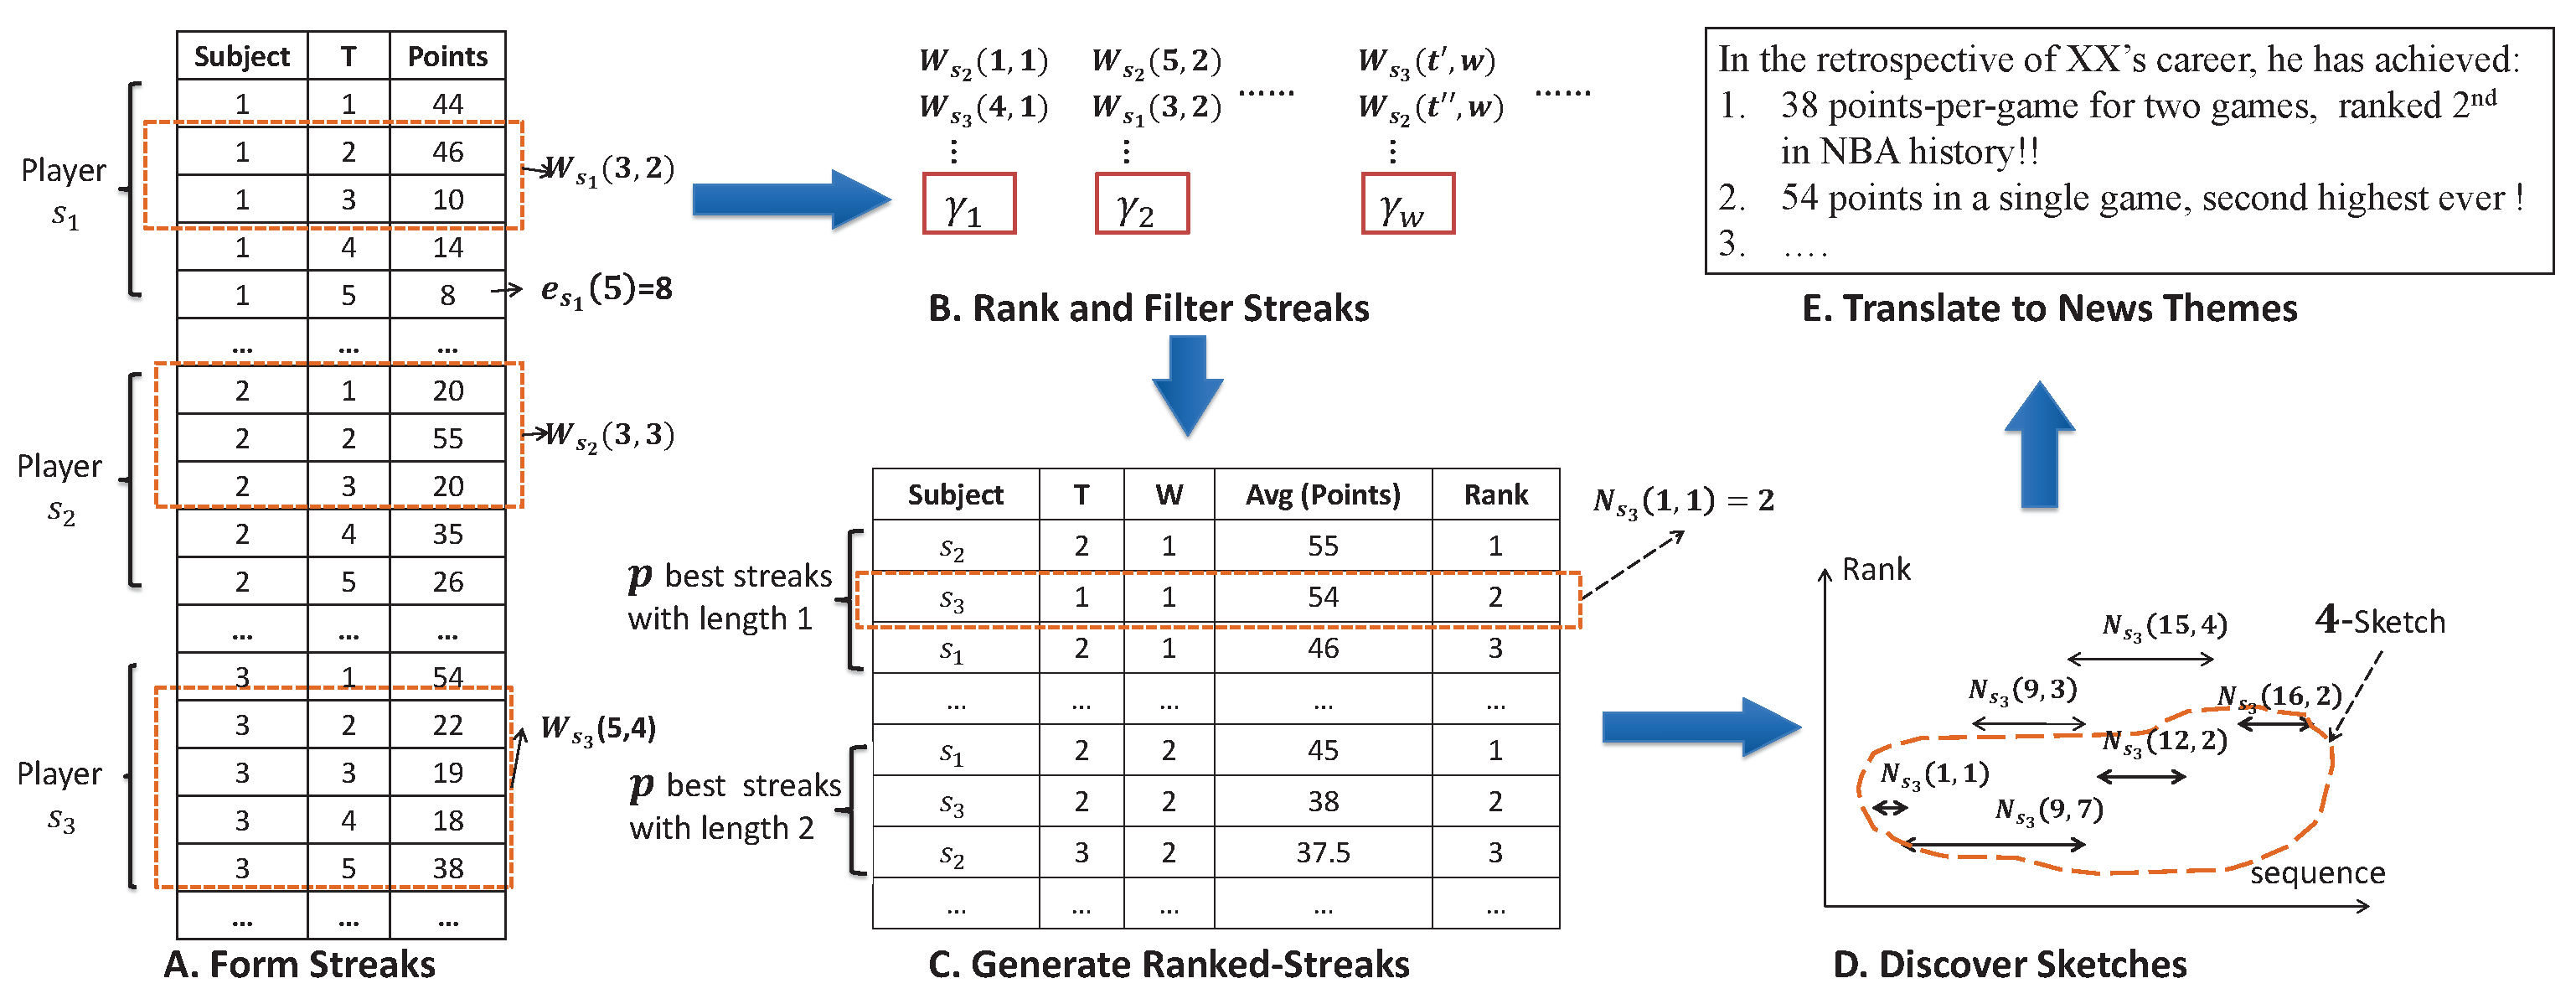
\includegraphics[width=1.0\textwidth]{chapter4/charts/application.eps}
	\caption{An illustration sketch discovery workflow. 
(A): various event windows are formed based on events' sequence IDs. 
(B): event windows with rank greater than $p$ are filtered.
(C): best ranked event windows form candidate themes.
(D): $k$-sketches are discovered for each subject from their candidate themes.
(E): subject related news can be generated from each $k$-sketch.
}
\label{fig:system_flow}
\end{figure*}

With the aggregated value $\overline{v}$, we can derive the rank of an event window, which can be used to measure the strikingness of an event window as a news theme.  For instance, ``\textit{The total points Kobe has scored is $32,482$}'' can be transformed into a rank-aware representation: ``\textit{Kobe moved into third place on the NBA's all-time scoring list}'', in which the rank is $3$. Let $W$ be a length-$w$ event window, and 
 $\gamma_w(W.\overline{v})$ be the rank of $W$ by comparing it with all other
length-$w$ event windows on their aggregate values. Generally speaking, an event window is newsworthy if its rank is smaller than a predefined threshold. This leads to our definition of \emph{Candidate Theme}:
%

\begin{definition} [Candidate Theme]
An event window $W_s(t,w)$ is said to be a candidate theme, denoted by $N_s(t,w)$, if its rank $\gamma_w(W_s(t,w).\overline{v}) \leq p$. $p$ is a user-defined threshold.

%which is a triple $\langle t, w, \gamma_w(W_s(t,w).\overline{v})\rangle$.
\end{definition} 

\begin{example}
In the step $(B)$ of Fig.~\ref{fig:system_flow}, we group the event windows based on their window length. Each window is associated with a rank value $\gamma_w$. If the rank value is greater than the threshold $p$, the associated event window is pruned. Otherwise, it is considered as a candidate. In the step $(C)$ of  Fig.~\ref{fig:system_flow}, we present the candidate themes  in the tabular format. Each candidate contains the rank computed from step (B). For instance, among all candidate themes with window length 1, $N_{s_3}(1,1)$ (with value $54$) is ranked 2nd because its aggregated value is smaller than that of another event window $N_{s_2}(2,1)$ (with value $55$). %Therefore the rank of $N_{s_3}(1,1).\gamma=2$.
\end{example}

Let $\mathbb{N}_s$ be the set of candidate themes of subject $s$. Since for each possible window length, there are at most $p$ candidate themes, the size of $\mathbb{N}_s$ can be as large as $p|\mathbb{H}_s|$, which is still overwhelming for news reporting.
To control the output size while maintaining the quality of news themes, we
aim to find, for each subject $s$, a small subset of $k$ 
candidate themes from $\mathbb{N}_s$. %, which $best$ describes $\mathbb{N}_s$. 
We call the subset  a $k$-\textbf{Sketch}. 

To measure the quality of a sketch, we define a scoring 
function $g(\cdot)$ over all sketches. The design of $g$ gives rise to two concerns.
First, $g$ needs to assign higher scores to the candidate themes with better ranks. This
is because better rank indicates good strikingness which implies that the news theme would
be more eye-catching. For instance, 
we can expect people to care more about who the top scorer in NBA history is rather than who ranked 20$^{th}$ in the history.
Second, $g$ prefers the sketches containing candidate themes with fewer overlapped events and avoids near-duplicate events. 
This is because near-duplicate themes generally do not add news values.
For example, when Kobe Bryant scored 81 points in a single game (2nd highest in NBA history),
all event windows containing that event are likely to have good and similar ranks. 
Thus, reporting all of them is not newsworthy.

To resolve these two concerns, we define $g$ as follows: given any set $\mathbb{X}_s$
of candidate themes about subject $s$ (i.e., $\mathbb{X}_s \subseteq \mathbb{N}_s$), 
the score of $\mathbb{X}_s $ is:
\begin{equation}
	\label{eq:scoring_function}
	g (\mathbb{X}_s) = \alpha C(\mathbb{X}_s) + (1-\alpha) R(\mathbb{X}_s), \alpha \in [0,1]
\end{equation}
where $C(\mathbb{X}_s)$ is the ratio between the number of distinct events covered by $\mathbb{X}_s$ 
over the total number of events about subject $s$. In this way, duplicated candidate themes 
contribute to a lower score. $R(\mathbb{X}_s) = \frac{1}{|\mathbb{X}_s|}\sum_{X_s \in \mathbb{X}_s} \frac{p-X_s.\gamma}{p}$ is the strikingness of $\mathbb{X}_s$. Any candidate themes in 
$\mathbb{X}_s$ changing to a better rank increases $R(\mathbb{X}_s)$. The values of $C(\mathbb{X}_s)$ and $R(\mathbb{X}_s)$ are normalized  between $[0,1]$. $\alpha$ is an adjustable coefficient to balance the weights between $C(\mathbb{X}_s)$ and $R(\mathbb{X}_s)$. If $\alpha$ is high, it means users are more interested in finding news themes that cover most of the subject's events.  If $\alpha$ is low, it indicates users prefer news themes whose ranks are small. 

With Equation~\ref{eq:scoring_function}, we then define the \emph{Sketch Discovery} problem as follows:

\begin{definition} [Sketch Discovery]
Given a parameter $k$, Sketch Discovery aims to, for each subject $s$, 
find a subset $SK_s$ from the candidate themes of $s$ (i.e., $SK_s \subseteq \mathbb{N}_s$), s.t. $|SK|_s = k$ and $g(SK_s)$ is maximized.
\end{definition}

\begin{example}  
In the step (D) of Fig.~\ref{fig:system_flow}, we show a collection of candidate themes and a $k$-sketch derived from them. The y-axis is the rank and the x-axis represents the complete sequence of events of a subject. Each candidate theme is represented by a line segment, covering a window of events. When $k=4$, four of the candidate themes are selected as a $4$-sketch as the most representative news for the subject.	
\end{example}

Before we move on to the algorithmic part, we first list the notations in Table~\ref{tbl:notations}. For the 
ease of presentation, we present our techniques using \emph{avg} as the default aggregate function in the following sections. Extending our techniques to other aggregate functions will be addressed in Section~\ref{sec:discussion}.

\begin{table}[h]
\centering
\begin{tabular}{|c|l|}
\hline 
\textbf{Notation} & \textbf{Meaning} \\ 
\hline
$S$ & set of subjects \\
\hline
$\mathbb{H}_s$ & set of events associated with subject $s$\\
\hline
$W_s(t,w)$ & length-$w$ event window of $s$ ending at $t$\\
\hline
$\mathbb{N}_s$ & set of candidate themes associated with subject $s$\\
\hline 
$N_s(t, w)$ & candidate theme derived from $W_s(t,w)$ \\ 
\hline 
$WI(w)$ & $p$ best ranked candidate themes of window length $w$\\
\hline
$\beta(w)$ & lower bound of $WI(w)$\\
\hline
$SK_s$ & sketch for subject $s$ \\
\hline
$J_s$ & visiting-window bound for subject $s$ \\
\hline
$M_s$ & unseen-window bound for subject $s$\\
\hline
$P_s$ & online-window bound for subject $s$\\
\hline
\end{tabular} 
\caption{Notations used in this chapter}
\label{tbl:notations}
\end{table}

\section {Offline Sketch Discovery}\label{sec:offline}
In the offline scenario, the input is a set of events
of all subjects and the output is a $k$-sketch 
for each subject $s$, denoted by $SK_s$. 
The sketch discovery process consists of two 
major steps: first generating the candidate themes of each subject (i.e., $\mathbb{N}_s$), 
and then discovering the sketches among those candidate themes. 

\subsection{Candidate Theme Generation}
Generating candidate themes for each subject is computationally 
expensive. In order to retain the candidate themes with rank no greater than $p$,
a brute-force approach needs to evaluate all the event windows with every possible length to generate accurate ranks. Since there could be $\mathbb{H}_s \choose 2$ event windows (with different lengths and ending sequence ids) associated with subject $s$, the total time complexity for the brute-force approach
is $O(\sum_{s \in S}|\mathbb{H}_s|^2)$. Such a complexity makes the solution infeasible even for moderate-sized datasets.

To improve the efficiency, 
we observe that it is not necessary to compute all the event windows to generate $\mathbb{N}_s$.
The intuition behind is that the upper bound value of event windows with longer lengths can be estimated from those
with shorter lengths. This means that we can compute event windows with increasingly lengths, and as the shorter event windows are computed, the longer event windows not in $\mathbb{N}_s$ can be pruned.
To realize such an intuition, we design the candidate generation algorithm
by adapting two novel window-based pruning methods which 
exploit the \emph{subadditivity} property among event windows with different window lengths.


\subsubsection{Overview of window pruning}
For each subject, its event windows can be grouped by window lengths. Our candidate
generation algorithm gradually evaluates a subject's event window from shorter
length to longer length. To support efficient pruning, 
we define two concepts, namely \emph{visiting-window bound} ($J_s$) and \emph{unseen-window bound} ($M_s$).
In particular, $J_s(w)$ is the upper bound of all the event windows about subject $s$ and with length $w$, i.e., $\forall w,J_s(w) \geq \max\{W_s(t,w).\overline{v} | t\in(0,w)\}$. 
$M_s(w)$ is the upper bound of all the event windows about subject $s$ with length larger than $w$, i.e., $M_s(w) \geq \max\{J_s(t) | t > w\}$.  These two bounds will be used for event window pruning and we will present how to estimate these two upper bounds in Sections~\ref{sec:visiting-window-bound} and~\ref{sec:useen-window-bound}.

%Utilizing these two bounds,
%we are able to design the \emph{visiting-window pruning} and \emph{useen-window pruning} techniques.

The overview of news theme generation algorithm is presented in Algorithm~\ref{algo:prune_overview}. We maintain two global structures $WI$ and $\beta$ (Lines~1-2). For each window length $w$, $WI(w)$ stores the top $p$ event windows with length $w$ among all the subjects and $\beta(w)$ is the $p$-th score among the candidates in $WI(w)$. 
In other words, $\beta(w)$ serves as a lower bound score. An event window with length $w$ is a candidate for the $k$-sketch only if its aggregate value is larger than $\beta(w)$. A priority queue $Q$ (Line 3) is used to provide an access order among the subjects. Each element in the queue is a triple $(s,w,q)$, where $s$ is a subject, $w$ indicates the next window length of $s$ to evaluate, and $q$ denotes the priority. We use the unseen-window bound (i.e., $M_s(w)$) as the priority during every iteration (Lines~13-14). Intuitively, an event window with higher $M_s(w)$ is more likely to spawn new event windows that can increase $\beta$ and benefit the subsequent pruning. During initialization, we insert, for each subject, an entry with window length $1$ and priority infinity into $Q$.

%the candidate with the maximum $M_s$ will be located on top of the priority queue. Intuitively, an event window with higher $M_s(w)$ is more likely to spawn new event windows that can increase the values in $\beta$ and facilitate the subsequent pruning. In the initialization step, we insert all the event windows with length $1$ into $Q$.

% and the comparison function in $Q$ is based on the value of $M_s$. C

%Instead of evaluating each subject one-by-one, we adapt a dynamic order of evaluation by using
%a priority queue $Q$ (Line 3). Each entry of the queue is a triple  where $s$ 
%is the subject, $w$ denotes the next length indicating that $s$'s event window with length $w$ are
%to be evalauted, $M_s$ is the unseen-window bound of $s$ which serves as an priority of the entry.
%The intuition of using $M_s$ as priority is that $M_s$ presents the potential maximum value of $s$.
%If $M_s$ is high, $s$ is likely to increase $\beta$. Higher $\beta$ brings higher pruning power.

In each iteration, we pop the event window with the highest priority (Line~\ref{code:subj_selection}). Then, we compute the visiting-window bound $J_s(w)$ for the subject and determine whether all the length-$w$ windows about subject $s$ can be pruned (Lines~\ref{code:v_prune_start}-\ref{code:v_prune_end}). If the bound $J(s)$ is no greater than $\beta(w)$, then all these event windows can be ignored. Otherwise, all the length-$w$ event windows of $s$ are computed to update $WI(w)$ and $\beta(w)$ accordingly (Lines~\ref{code:e_compute_start}-\ref{code:e_compute_end}).
% We also update $J_s$ as the maximum score among these event windows. 
In the next step, we estimate the unseen-window bound $M_s$ and compare it with the minimum $\beta(w')$ for all $w'> w$. If $M_s$ is smaller, then we would not find a better candidate and all the event windows about subject $s$ and with length larger than $w$ can be pruned (Lines~\ref{code:u_prune_start}-\ref{code:u_prune_end}). Otherwise, we assign $M_s$ to the priority $q$, and push the triple $(s,w+1,q)$ back into the queue (Lines~13-14). The algorithm terminates when all the candidates have been evaluated and $Q$ becomes empty.
%$\beta$s can be organized as an Interval Tree~\cite{Berg1997Computational} so that such comparison
%is efficiently supported. If the unseen-window pruning fails, the triplet $(s,w+1,M_s)$ 
%is inserted back to $Q$ (Lines~\ref{code:q_insert}). 

%Instead of evaluating each subject one-by-one, we adapted a dynamic order of evaluation as
%follows: We maintain a priority queue $Q$ (Line 3). Each subject is assigned with a triple
%$\langle s, w, M_s(w) \rangle$ as the queue state, where $w$ refers to the next window-length to
%be evaluated of subject $s$ and $M_s(w)$ is the \emph{unseen-window bound}. The value $M_s(w)$
%is served as the priority of the triple. 
%During our algorithm, we pick one state in every 
%iteration (Lines 4-17). Then we compute the length-$w$ event windows of subject $s$. We use \emph{visiting-window}
%bound $J_s$ (Lines 5-6) to decide whether to evaluate the event windows with length $w$ of subject $s$. Then
%we use \emph{unseen-window bound) $M_s$ (Lines 13-14) to decide whether to insert $s$ with updated state back to queue.

%The intuition of using $M_s$ as the priority is that subject with higher $M_s$ values is likely to contribute %


%Instead of enumerating every possible event window to produce $\mathbb{N}_s$, 
%our candidate theme generation algorithm iteratively picks a subject $s$ based and 
%examines its event windows whose length has not been evaluated yet.
%We develop two types of pruning techniques: \emph{visiting-window} pruning
%and \emph{unseen-window} pruning. The former can avoid evaluating event windows with length $w$ while the latter avoids evaluating event windows with length greater than $w$.

\begin{algorithm}[t]
\caption{Candidate Theme Generation Overview}
\label{algo:prune_overview}
\begin{algorithmic}[1]
\State $WI() \gets \{\}$ // $p$ best event windows for each window length
\State $\beta \gets \{\}$ // smallest scores in $WI$ for each window length
\State $Q \gets \{(s,1,+\infty) | s \in S\}$
\While{$(s,w,q) \gets Q.pop()$} \label{code:subj_selection}
	%	\State $w \gets w+1$
%		\State $J_s(w) \gets \frac{J_s(1) + (w-1)J_s(w-1)}{w}$ \label{code:v_prune_start}
		\State compute $J_s(w)$	\label{code:v_prune_start}	
		\If{ $J_s(w) > \beta(w)$} \label{code:v_prune_end}
			\For{$t \in w...|\mathbb{H}_s|$}\label{code:e_compute_start}		
				\State Update $WI(w)$, $\beta(w)$, and $J_s(w)$
%				\State $J_s(w) \gets \max(J_s(w),W_s(t,w).\overline{v})$			
			\EndFor	\label{code:e_compute_end}
%			\State $J_s(w) \gets \max\{W_s(t,w) | t\in [w, \mathbb{H}_s] \}$ 
		\EndIf
%		\State $M_s \gets J_s(w) +\min\{\frac{1}{2}J_s(1),\frac{w-1}{w+1}J_s(w-1)\}$ \label{code:u_prune_start}
		\State compute $M_s(w)$ whose value relies on $J_s(w)$\label{code:u_prune_start}
		\If{$M_s(w) > \min\{\beta(w')|w < w' \leq |\mathbb{H}_s|\}$} \label{code:u_prune_end}
			\State $q \leftarrow M_s(w)$
			\State $Q.push(s,w+1,q)$ \label{code:q_insert}
		\EndIf
\EndWhile \\
\Return $WI$
\end{algorithmic}
\end{algorithm}

%The overview of our candidate theme generation algorithm is shown 
%in Algorithm~\ref{algo:prune_overview}. In the algorithm,
%$WI$ is a set of min-heaps and $WI(w')$ tracks the $p$ best event windows with length $w'$ among all the subjects.
%We use $\beta(w')$ to denote the $p$-th score for event windows in $WI(w')$.
%$Q$ is a priority queue to maintain the subject evaluation order, where $M_s$ (as explained next) 
%is used to indicate the priority value.

%$\beta$ is the set of scores where $\beta_w$ maintains the smallest aggregation 
%value of event windows in $WI(w)$.
%$Q$ is a priority queue which maintains the subject access order. 
%Each entry in $Q$ is a triplet $(s,w,M)$ where $s$ is the subject ID, 
%$w$ is the window length such that event windows with length larger 
%than $w$ have not been evaluated yet, and $M$ is the priority of the entry in $Q$.

%We also keep $M_s(w)$ for each $s$ to be the upper bound
%for the aggregate scores of all $s$'s event windows with length $> w$.
%That is $M_s(w) \geq max_{w' \in (w, \mathbb{H}_s]}J_s(w')$. $J_s$ and $M_s$ are
%used for visiting-window and unseen-window prunings.

%\subsubsection{Subadditivity on event windows}
%Before we introduce the estimation of $J_s(w)$ and $M_s(w)$, we present an important concept named subaddivity property, which is helpful for the upper bound estimation.

%As visiting-window pruning and unseen-window pruning rely on $J_s(w)$ and $M_s$, 
%it is vital to derive the $J_s(w)$ and $M_s(w)$ effectively and efficiently. We observe
%that $J_s(\cdot)$ has the subaddivity property, which my leads to tight values of both $J_s$ and $M_s$.
%Before we moving on to the derivations, let us first prove the subadditivity property of $J_s(\cdot)$
%as stated in the following theorem:
%Before moving on to the derivation
%on these two values, we first prove the following theorem which serves as a basis of the deductions.
%\begin{theorem}[Subadditivity]
%\label{thm:subadditivity}
%Let $J_s(w)$ be the visiting-window bound (i.e., $J_s(w) \geq \max\{W_s(\cdot,w).\overline{v}\})$ then there exists a non-decreasing
%function $U(\cdot,\cdot)$~\footnote{Non-decreasing means for two pairs $(x_1,y_1)$, $(x_2,y_2)$, if $x_1 \leq x_2$ and $y_1 \leq y_2$ then $U(x_1,y_1) \leq U(x_2,y_2)$} such that the following equation holds:
%\begin{equation}
%J_s(w) \leq U(J_s(w_i), J_s(w-w_i)), \forall w_i \in (0,w)
%\end{equation}
%\end{theorem}
%We prove the theorem by constructing such $U(\cdot,\cdot)$s. We demonstrate the proof
%for \emph{avg} as stated in the following lemma:

% The respective
%constructions for other aggregate functions can be found in the Section~\ref{sec:discussion}.

%\begin{lemma}[Average Subadditivity]
%\label{lem:subaverage}
%Let $\overline{J}_s(w)$ be the best score of all $s$'s event windows with length $w$, then the following
%equation holds:
%\begin{equation}
%\small
%\label{eq:subadditivity}
%	\overline{J}_s(w) \leq \frac{w_1 \overline{J}_s(w_1) + (w-w_1) \overline{J}_s(w-w_1)}{w}, \forall w_1 \in (0..w)
%\end{equation}
%\end{lemma}
%\begin{proof}
%Let $\overline{J}_s(w)$ correspond to the event window $W=W_s(t,w)$, 
%i.e., $W.\overline{v}= \Sigma_{e \in W}e/w$. Given a $w_1 \in (0,w)$,
%we can split $W$ into two non-overlapping event windows with lengths $w_1$ and $w-w_1$,
%i.e.,$W_1 = W_s(t,w_1)$ and $W_2 = W_s(t-w_1, w-w_1)$. Due to the non-overlapping of $W_1$ and $W_2$,
%it follows that $wW.\overline{v} = w_1W_1.\overline{v} + (w-w_1)W_2.\overline{v}$. 
%Since $\overline{J}_s(\cdot)$ is best score, it follows that 
%$\overline{J}_s(w)=(w_1W_1.\overline{v} +(w-w_1)W_2.\overline{v})/w \leq (w_1\overline{J}_s(w_1)+ (w-w_1)\overline{J}_s(w-w_1))/w$.
%\end{proof}

\subsubsection{Visiting-window pruning}  
\label{sec:visiting-window-bound}
In Algorithm~\ref{algo:prune_overview}, we need to compute the visiting-window bound $J_s(w)$ to facilitate pruning all length-$w$ event windows associated with subject $s$. Our idea is that suppose we have successfully derived the bounds for windows with smaller lengths, we can use them to estimate the bounds of larger windows. We formulate it as the subadditivity property and use $avg$\footnote{Although here we demonstrate the bound
using ``avg'', the properties and bounds also hold for other aggregate functions. Corresponding properties and bounds for other aggregate functions are listed in Section~\ref{sec:discussion}.
} as the aggregate function for illustration: 

\begin{theorem}[Subadditivity (for $avg$)]
\label{lem:subaverage}
\begin{equation}
\small
\label{eq:subadditivity}
	\max_t\{W_s(t,w).\overline{v}\} \leq \frac{w_i J_s(w_i) + (w-w_i) J_s(w-w_i)}{w}, \forall w_i \in (0,w)
\end{equation}
\end{theorem}
\begin{proof}
Given any event window $W=W_s(t,w)$ with length $w$ and a value $w_i \in (0,w)$, we can split the window into two non-overlapping sub-windows with lengths $w_i$ and $w-w_i$, i.e.,$W_1 = W_s(t,w_i)$ and $W_2 = W_s(t-w_i, w-w_i)$. Due to the non-overlapping property of $W_1$ and $W_2$, we have $wW.\overline{v} = w_iW_1.\overline{v} + (w-w_i)W_2.\overline{v}$.  Since $J_s(w_i)$ and $J_s(w-w_i)$ are two visiting-window bounds, we have $W_1.\overline{v}\leq J_s(w_i)$ and $W_2.\overline{v}\leq J_s(w-w_i)$. %for the $avg$ operator
Then, we complete the proof and $\frac{w_i J_s(w_i) + (w-w_i) J_s(w-w_i)}{w}$ is a bound for event windows with length $w$.
\end{proof}


%The proofs of other aggregate functions will be presented in Section~\ref{}.


%\begin{example}
%The subadditivity property of $J_s$ can be understood intuitively. 
%Let us consider $J_s(1)$ and $J_s(2)$ in an NBA application,  where $J_s(w)$ refers to a player's best average score of %consecutive $w$ games. It is easy to see that, for any player, his best average score for consecutive two games (i.e., $J_s(2)$) %cannot exceeds his best average score for a single game (i.e., $J_s(1)$). That is $J_s(2) \leq \frac{J_s(1)+J_s(1)}{2}$ as in our %theorem. Numeric examples can be found in Figure~\ref{fig:window_pruning}, where we can validate that
%$J_s(2)= 39.5$ while $J_s(1)=42.0$. A more complex example is also available, such as $J_s(5)= 31.8$, while $\frac{J_s(3) * 3 + %J_s(2) * 2}{5} = 36.9$.

%and $J_s(3)$ in the NBA application, where $J_s(t)$ refers to a player's best average score of consecutive $t$ games.
%Given the best three games the player played, (i.e., $J_s(3)$), in the first game, the player cannot score better than $J_s(1)$. This is because $J_s(1)$ represent the best single game score of that player. Similarly, in the remaining two games,
%the player cannot obtain an average score better than $J_s(2)$. Therefore, in total, $J_s(3) \leq \frac{J_s(2) * 2 + J_s(1)}{3}$.
%\end{example}

%Based on the \emph{Subadditivity} on $J_s(\cdot)$,
%we are ready to devise the ``visiting-window'' and ``unseen-window'' pruning as in the following sections.
%we are able to derive the $J_s(\cdot)$ and $M_s(\cdot)$
%for `visiting-window' pruning and `unseen-window' pruning. 
%In the remaining parts of this section, we illustrate the two pruning 
%techniques using \emph{avg} as the aggregate function. The respective bounds of other aggregate functions
%are described in the Section~\ref{sec:discussion}.


With Theorem~\ref{lem:subaverage}, we can estimate $J_s(w)$ by any pair $J_s(w_1)$ and $J_s(w-w_1) $, $\forall w_1 < w$. 
To derive a tighter bound for $J_s(w)$, we formulate the following optimization problem:
%
\begin{equation}  
\label{eq:cw_mini_1}
w_1 = \argmin_{t \in (0,w)}\frac{J_s(t)*t + J_s(w-t) *(w-t)}{w}
\end{equation}

A naive solution would enumerate every possible $t$ 
to get the tightest bound. However, such a solution 
has a worst time complexity of $O(|\mathbb{H}_s|)$ for subject $s$. 
To quickly compute $w_1$ without compensating the running time,
we apply a continuous relaxation to Eqn.~\ref{eq:cw_mini_1} as follows: 
Let $G_s(t) = J_s(t) * t \;\;\forall t$, 
then Eqn.~\ref{eq:cw_mini_1} is equivalent to:
%To quickly retrieve a tight bound without compensating running time, 
%we design a $O(1)$ estimation of $J_s(w)$ as follows: Let $G_s(t) = J_s(t) * t \;\;\forall t$, 
%then Eqn.~\ref{eq:cw_mini_1} is equivalent to:
\begin{equation}
\label{eq:cw_mini_2}
w_1 = \argmin_{t\in 1..w-1} \{G_s(t) + G_s(w-t)\}
\end{equation}
Let $L_s(t)$ be a continuous and smooth fitting function 
of $G_s(t)$ for $t \in [1,w-1]$.  Eqn.~\ref{eq:cw_mini_1} can then be relaxed by replacing $G_s(t)$ with $L_s(t)$ to produce
the solution at $w_1=w/2$ if $L_s(t)$ is convex and $w_1=1$ 
if $L_s(t)$ is concave. We have observed, over all aggregate functions, the convexity and concavity for $L_s(\cdot)$
when approximating $G_s(\cdot)$. 
%The continuous relaxation of 
%Eqn.~\ref{eq:cw_mini_2} has the solution at $w_1=w/2$ 
%if $L_s(t)$ is convex and $w_1=1$ if $L_s(t)$ is concave. 
%By the observations over all aggregate functions, 
%we confirm the convexity and concavity
%for $L_s(\cdot)$ when approximating $G_s(\cdot)$.
For example, we use 800 games of a NBA player and plot the 
function $G_s$ and $L_s$ under various aggregate functions in Figs.~\ref{fig:convex_exp}. 
In Fig.~\ref{fig:convex_exp}(a), $G_s$ and $L_s$ for \emph{min} and \emph{avg} are presented. 
We can see that the fitting $L_s$ for \emph{min} is convex while that for $avg$ is concave.
Similarly, in Fig.~\ref{fig:convex_exp}(b), 
we can see that $L_s$ is concave for count, sum and max. 
In the worst-case scenario, even when $L_s(\cdot)$ is neither convex nor concave, 
$J_s(w) < \frac{J_s(1) + (w-1)J_s(w - 1))}{w}$ still holds due to 
Theorem~\ref{lem:subaverage}. Thus we have the visiting-window bound stated as:

\begin{theorem}[Visiting-Window Bound]
\label{thm:visiting_window_bound}
Given a window length $w > 1$, let $J_s(w)$ be:
\begin{equation}
J_s(w) = \frac{J_s(1) + (w-1)J_s(w-1)}{w}
\end{equation}
then $J_s(w)$ is a visiting-window bound, i.e. $ J_s(w) \geq \max_t$ $W_s(t,w).\overline{v}$
\end{theorem}
%\begin{proof}
By substitute $w_i = 1$ to the r.h.s. of Theorem~\ref{lem:subaverage}, we see this theorem holds. 
%\end{proof}

In Algorithm~\ref{algo:prune_overview}, $J_s(w)$ is computed incrementally. Initially, $J_s(1)$
is set as the single event of $s$ with highest value. Then, as the subject $s$ is processed,
$J_s(w)$ is computed by Theorem~\ref{thm:visiting_window_bound}. In the case that $J_s(w)$ is not 
pruned, we may assign $J_s(w)$ with the maximum length-$w$ event window of $s$ to further tighten
the bound. 

%To use the recursive form of visiting-window bound in Theorem~\ref{thm:visiting_window_bound}, $J_s(1)$ 
%can be easily obtained by find the event window with greatest aggregate value. During Algorithm~\ref{algo:prune_overview},
%we always maintain an $J_s(w)$ for every computed window lengths. If $J_s(w)$ is pruned, we use Theorem~\ref{thm:visiting_window_bound} to obtain $J_s(w)$. If the visiting-window pruning fails, we set $J_s(w)$
%to be the maximum value among event windows of size $w$. 
%Although Theorem~\ref{lem:subaverage} demonstrate the subadditivity for ``average'' function,
%the properties holds for other aggregate functions as well. We list the subaddivity and visiting-window
%bound for other aggregate functions in Section~\ref{sec:discussion}.


%PLEASE MAKE A SUMMARY OF HOW TO ESTIMATE THE UPPER BOUND IN DIFFERENT SCENARIOS. ALSO NEED TO ADDRESS HOW TO ESTIMATE $J_s(1)$. ANOTHER CASE IS WHAT HAPPENS IF window length w-1 IS PRUNED. THEN, HOW TO ESTIMATE $J_s(w-1)$

%\begin{theorem}[Visiting-Window Bound]
%\label{thm:visiting_window_bound}
%Let $J_s(w)$ be:
%Let $J_s(w)$ \geq \max $ $\{W_s(t,w).\overline{v} | t\in (0,w]\}$, then $J_s(w)$
%is estimated as:
%Given a $J_s(w)$ as:
%\begin{equation}
%J_s(w) = \frac{J_s(1) + (w-1)J_s(w-1)}{w}
%\end{equation}
%$J_s(w)$ is a visiting-window bound, i.e. $\forall t \in (0,w], J_s(w) \geq W_s(t,w).\overline{v}$
%where $J_s^*(\frac{w}{2}) = max\{J_s(\lfloor \frac{w}{2} \rfloor), J_s(\lfloor \frac{w}{2} \rfloor + w \text{ mod } 2)\}$. 
%\end{theorem}
%\begin{proof}
%We may see the correctness of the Theorem by setting $w_i$ to $1$ in Theorem~\ref{lem:subaverage}.
%From Lemma~\ref{lem:subaverage}, we see $J_s(w) \leq \frac{J_s(1) + (w-1)J_s(w-1)}{w}$. 
%We show $J_s(w) \leq J_s^*(\frac{w}{2})$ as follows:\\
%When $w$ is even, $J_s(w) \leq J_s(\frac{w}{2}) \leq J_s^*(\frac{w}{2})$. \\
%When $w$ is odd,  $J_s(w) \leq  \frac{\lfloor \frac{w}{2} \rfloor J_s(\lfloor \frac{w}{2} \rfloor)
%+ (\lfloor \frac{w}{2} \rfloor+1)J_s( \lfloor \frac{w}{2} \rfloor+1)}{w}\leq \frac{\lfloor \frac{w}{2} \rfloor J_s^*(\frac{w}{2})
%+ (\lfloor \frac{w}{2} \rfloor+1)J_s^*(\frac{w}{2})}{w} = J_s^*(\frac{w}{2})$, which leads to the theorem.
%\end{proof}
%The visiting-window bounds for other aggregate functions are described in Section~\ref{sec:discussion}.

\begin{figure}
	\centering
    \begin{subfigure}[b]{0.45\textwidth}
        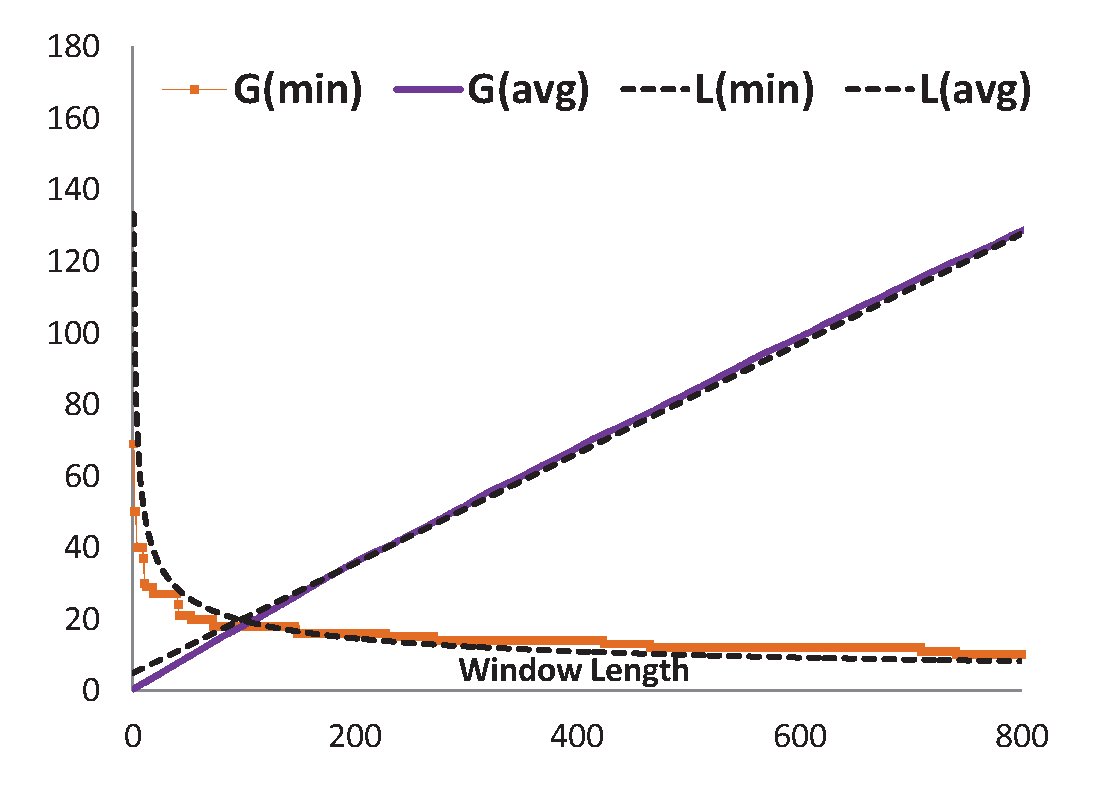
\includegraphics[width=\textwidth]{chapter4/charts/convex.eps}
        \caption{}
%        \label{fig:active_update}
    \end{subfigure}
    \begin{subfigure}[b]{0.45\textwidth}
        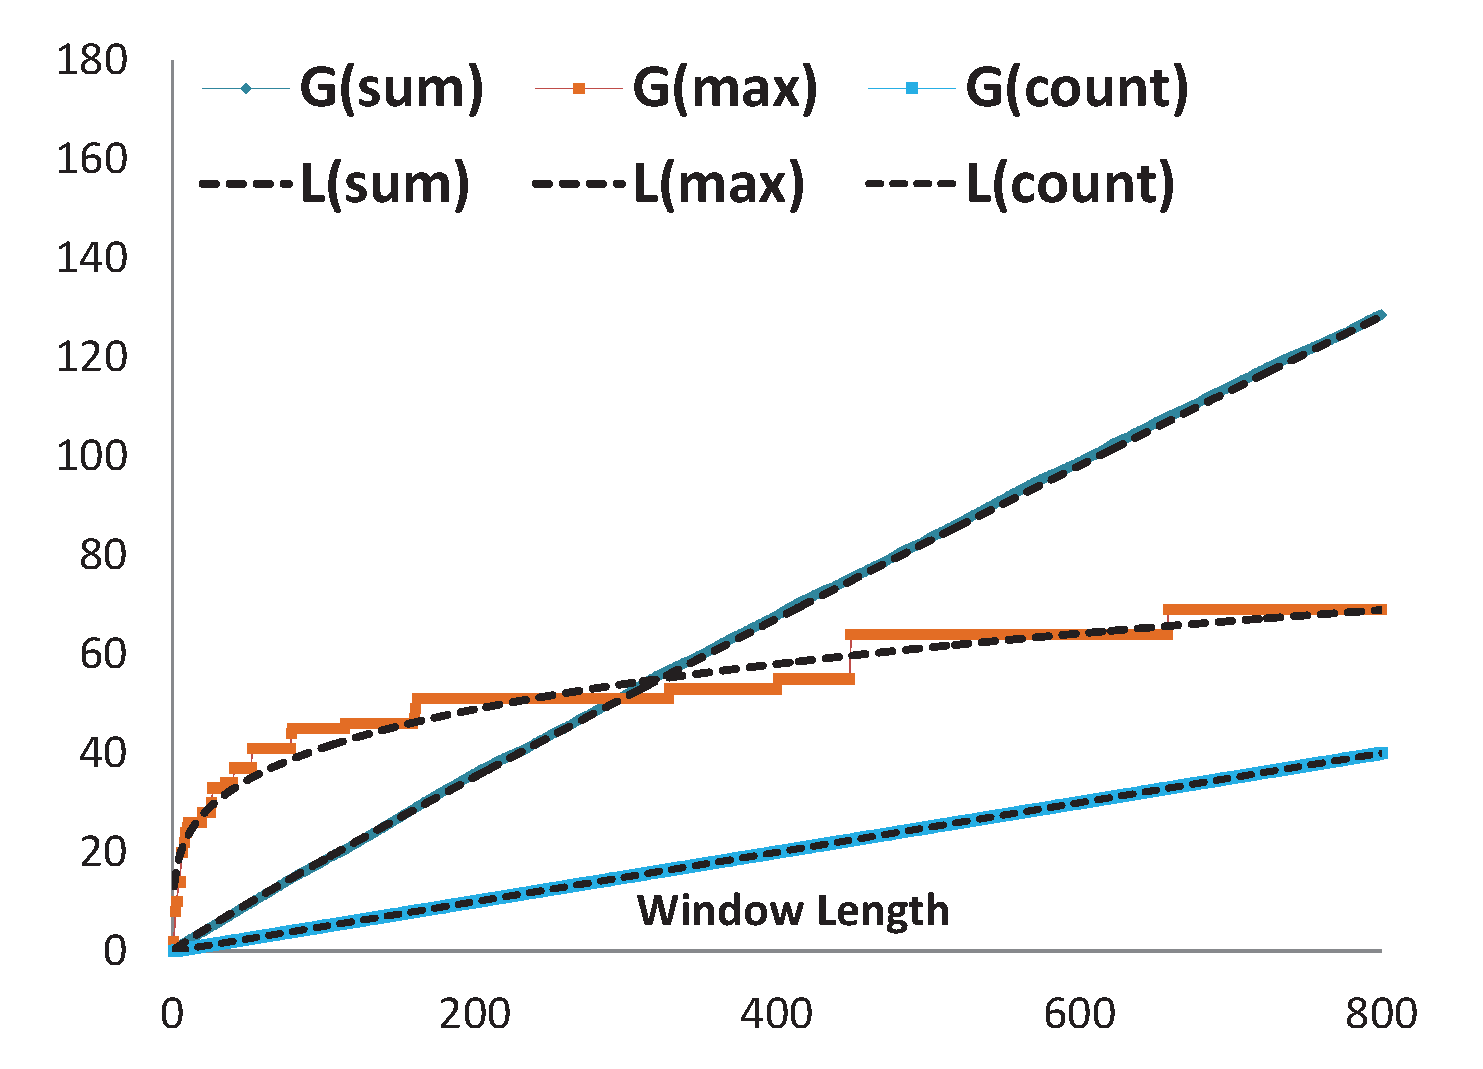
\includegraphics[width=\textwidth]{chapter4/charts/concave.eps}
        \caption{}
%        \label{fig:passive_update}
    \end{subfigure}
    \caption{Illustration of fitting function $L$ on various aggregation functions; solid lines represent $G$ while dotted lines represent $L$. (a) fitting on min and average (b)fitting on max,sum and count.}
    \label{fig:convex_exp}
\end{figure}


\subsubsection{Unseen-window pruning}
\label{sec:useen-window-bound}
Unseen-window pruning utilizes $M_s(w)$ to check if it is necessary to evaluate any 
window $w' \in (w,|\mathbb{H}_s|]$. We observe that $M_s(w)$ can
be efficiently estimated from the values of $J_s(w')$, where $w'\leq w$. 
For example, when $avg$ is used as the aggregate function, $J_s(1)$ is obviously an upper bound for $M_s(w)$ because $J_s(1)$ is essentially the maximum event value. However, such an upper bound is very loose. By utilizing the following theorem, we can derive a tighter bound as follows:

\begin{theorem}[Unseen-Window Bound]
\label{thm:unseen_window_bound}
Given that $J_s(1),$ ..., $J_s(w-1)$ have already been computed, 
%let $M_s = \max\{J_s(t),$ $t\in [w,|\mathbb{H}_s|]\}$,  
%then $M_s$ is estimated as:
let $M_s(w)$ be:
\begin{equation}
M_s(w) = J_s(w) + \min\{\frac{1}{2}J_s(1),\frac{w-1}{w+1}J_s(w-1)\}
\end{equation} 
then $M_s(w)$ is an \emph{unseen-window bound}, i.e. $M_s(w) \geq \max\{J_s(t) | $ $ t\in [w,|\mathbb{H}_s|]\}$
\end{theorem}
\begin{proof}
First, given any integer $k \geq 1$, we see that $J_s(kt) \leq J_s(t)$ 
by making use of Lemma~\ref{lem:subaverage} in a simple induction proof. 
Then, for any integer $x > w$, 
$x$ can be written as $x =\lfloor \frac{x}{w} \rfloor w + x \text{ mod } w$. 
Based on the subadditivity of $J_s(\cdot)$, we have: 
\begin{align*}
J_s(x) &\leq \frac{(\lfloor \frac{x}{w}  \rfloor *w) J_s(\lfloor \frac{x}{w}  \rfloor*w) + (x \text{ mod } w ) J_s(x \text{ mod } w)}{x} \\
&\leq J_s(\lfloor \frac{x}{w}  \rfloor*w) + \frac{x \text{ mod } w}{x} J_s(x \text{ mod } w) \text{, $\lfloor \frac{x}{w}  \rfloor * w \leq x $} \\
&\leq J_s(w) + \frac{x \text{ mod } w}{x} J_s(x \text{ mod } w) \text{, $J_s(kt) \leq J_s(t)$ }
\end{align*}
On one hand, since $t*J_s(t)$ is a monotone increasing function, it follows $(x \text{ mod } w)J_s(x \text{ mod } w) \leq (w-1)J_s(w-1)$. 
Moreover, since $x \geq w+1$, we have $(x \text{ mod } w)\frac{J_s(x \text{ mod } w)}{x}\leq (w-1)\frac{J_s(w-1)}{w+1}$. On the other hand, $J_s(x \text{ mod } w)\leq J_s(1)$ and $\frac{x \text{ mod } w}{x} \leq \frac{1}{2}$ for $x > w$, we have $(x \text{ mod } w)\frac{J_s(x \text{ mod } w)}{x} \leq \frac{1}{2}J_s(1)$.
Then it naturally leads to Theorem~\ref{thm:online_bound}. 
\end{proof}

%The unseen-window bound for other aggregate functions can be derived using similar techniques and 
%the bounds are described in Section~\ref{sec:discussion}.

To utilize $M_s(w)$, after the derivation, we check if $M_s(w)$ is no greater  
than any $\beta(w')$ with $w' >w$,  i.e. $M_s(w) \leq \min\{\beta(w')|w' \in (w ,|\mathbb{H}_s|]\}$. Whenever the condition holds, it is safe to stop further evaluation on subject $s$.
Note that we may maintain an interval tree~\cite{Berg1997Computational} 
on $\beta$ to support efficient checking. 

\begin{theorem}
\label{thm:window_prune}
Each candidate theme returned by Algorithm \ref{algo:prune_overview} has a rank no greater than $p$. 
\end{theorem}
The proof is quite straightforward according to the descriptions for Algorithm~\ref{algo:prune_overview}, visiting-window and unseen-window pruning. Thus, the details are omitted.

\begin{figure}[t]
\centering
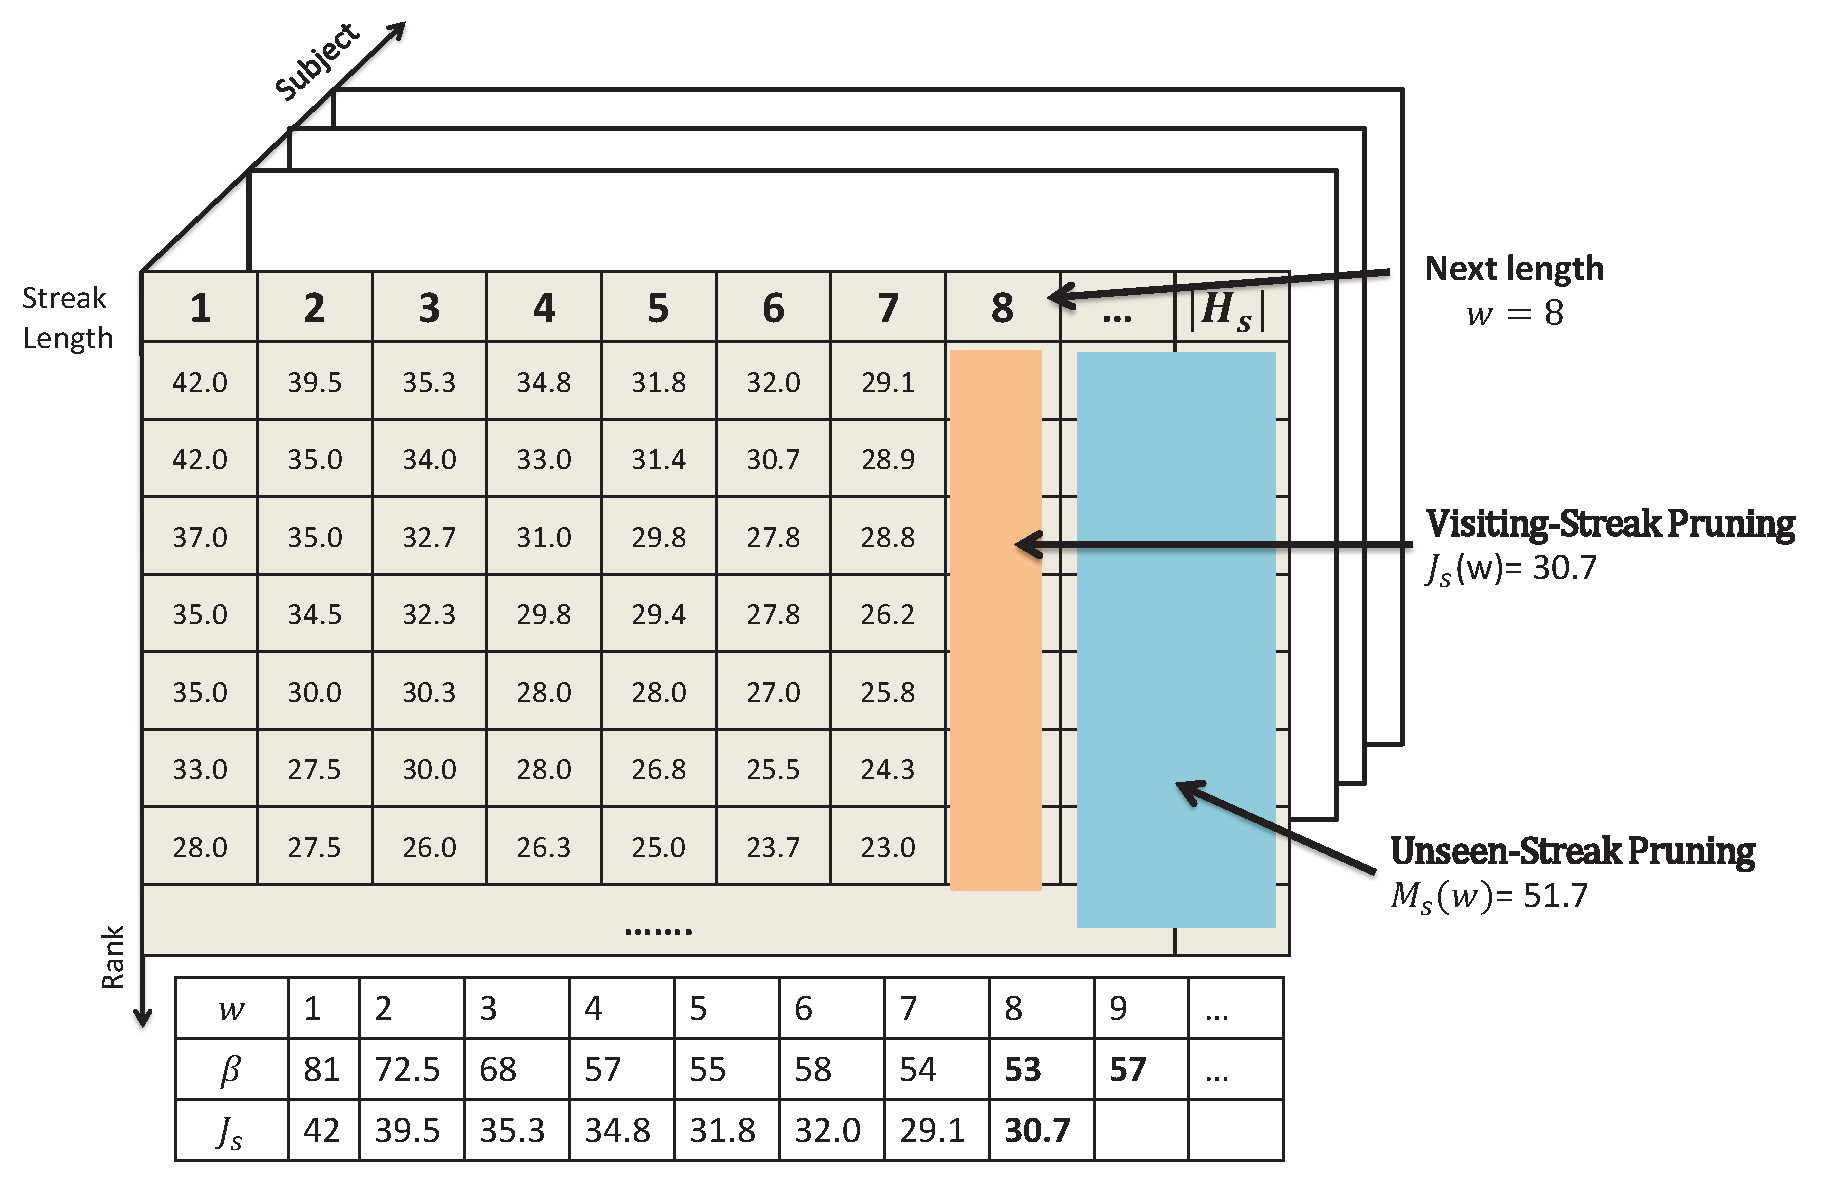
\includegraphics[width=\textwidth]{chapter4/charts/window_pruning.eps}
	\caption{An illustration of window-level pruning techniques. Each square slice represents a
	set of event windows to be computed for a subject, where the column represents window length and the row represents
	the rank. The value in each cell is the aggregate result (i.e., $\overline{v}$) for the corresponding event window.}
\label{fig:window_pruning}
\end{figure}

\begin{example}
We use Fig.~\ref{fig:window_pruning} to illustrate our pruning techniques on a subject $s$.  Each column in the table represents a window length and the cells contain the average values among different event windows with different lengths. For example, the cell in the second row and third column refers to the second largest average value among the event windows with length $3$. Algorithm~\ref{algo:prune_overview} essentially accesses the event windows in increasing order of the window length. Suppose we are about to estimate the upper bound for event windows with length $8$. At this point, the values of $\beta$ and $J_s$ are depicted in the figure. Then, our first job is to estimate the upper bound for all the average values in the $8$-th column.  Based on the values of $J_s(w)$ on smaller windows, we estimate $J_s(8) = \frac{42+7*29.1}{8}= 30.7125$. Since $J_s(8) < \beta(8)$, we can safely prune the whole column, as highlighted in the figure. Afterwards, we estimate the upper bound for all the windows with length larger than $8$. The value of $M_s(8)$ is then estimated as $M_s(8)= 30.7125 + \min\{21, \frac{7}{9}*29.1\}=51.7$. Since all the values of $\beta$ are greater than $M_s(8)$, it is safe to terminate the event window enumeration.
\end{example}

\subsection{Sketch Computation}
After the candidate themes are obtained,
the second step of the sketch discovery process is to, for each subject $s$, extract 
$k$ themes to form sketches $SK_s$ to maximize Eqn.~\ref{eq:scoring_function} (i.e., $g$). 

Our goal of optimizing $g$ is related to the Partly Interval Set Cover (PISC) problem. The goal in PISC is to select a set
of intervals which covers at least a certain percentage of elements. If no rank value is considered in $g$ (i.e., $\alpha = 1$), the
solution in~\cite{golab2009sequential} for PISC maximizes $g$ in $O(\mathbb{H}_s^3)$ time for each subject $s$. However, when
the rank is considered (i.e., $0< \alpha < 1$), optimizing $g$ becomes an open problem as stated in~\cite{edwards2013partial}, where current polynomial time solutions remain unknown.
%
% In PIMC, the ground set contains $n$ points. The input of PIMC is a set of intervals, and a ratio $r$. The goal of PIMC is to find the minimum number
%of intervals which collectively covers at least $rn$ points. The exact methods for solving PIMC takes $O(n^2)$ as stated in~\cite{edwards2013partial}. To use (PIMC) to solve sketch discovery, we may model a candidate theme as an interval, and events of a subject as points.
%Then we may invoke PIMC solution with a $r$ value to find the minimum set of intervals which covers $r\mathbb{H}_s$ events. 
%By examine all possible $r$ values, we are able find the set of intervals maximizing $g$. However, this approach takes $O(\mathbb{H}_s^3)$ time complexity, which is not scalable.
%%NEED TO FURTHER VERIFY
%A related problem to optimizing $g$ is the Partly Interval Max-k Cover problem, where the current best known exact solution~\cite{edwards2013partial} has a quadratic complexity.
To facilitate scalable sketch discovery, we provide 
an efficient $(1-1/e)$ approximation algorithm by exploiting the submodularity property\footnote{A function $I$ is submodular if and only if given two set $A \subseteq B$ and
an element $x \not\in B$, then $I(A \cup \{x\}) - I(A) > I(B \cup \{x\}) - I(B))$.} of the scoring function. Our idea is that since $g$ is not submodular, it is not easy to directly maximize it. However, by applying a relaxation on $g$, we are able
to gain a submodular function $g'$ s.t. maximizing $g'$ would result in
the same optimal solution as maximizing $g$. We design the function of $g'$ as follows:
\begin{equation}
\label{eq:gscore}
g'(\mathbb{X}_s) = \eta_1C'(\mathbb{X}_s) + \eta_2R'(\mathbb{X}_s)
\end{equation}
where $C'(\mathbb{X}_s)$ is the number of distinct events covered by $\mathbb{X}_s$,
 $R'(\mathbb{X}_s) = \Sigma_{X_s \in \mathbb{X}_s}(p-X_s.r)$, $\eta_1 = \alpha/|\mathbb{H}_s|$
and $\eta_2 = (1-\alpha)/k$. Given $k$, $s$ and $g$,
$g'$ is uniquely defined. We have the following theorem which links $g'$ to $g$:

\begin{theorem}
If $A^*$ is the optimal solution wrt. $g'$, then $A^*$ is
also the optimal solution wrt. $g$.
\end{theorem}
\begin{proof}
First observe that, for any set $A \subseteq \mathbb{N}_s$ of size $k$, (i.e., $|A|=k$),
$g(A) = g'(A)$. This can be validated by substituting $A$ into Eq.~\ref{eq:scoring_function} and Eq.~\ref{eq:gscore}. Then,
we prove the theorem by contradiction: 
If $A^*$ is not optimal wrt. $g$, then $\exists B^*$ s.t. $g(B^*) > g(A^*)=g'(A^*)$. However,
since $|B^*|=k$, $g'(B^*)=g(B^*) > g'(A^*)$, which contradicts with $A^*$'s optimality w.r.t. $g'$.
\end{proof}

Henceforth, we are able to compute sketches by maximizing $g'$ instead of $g$. 
We then prove the \emph{submodularity} on $g'$ as stated below:
\begin{theorem}
\label{thm:submodular}
Given a candidate theme set $\mathbb{X}_s$,
$g'(\mathbb{X}_s)$ is submodular.
\end{theorem}
\begin{proof}
Note that $C'$ is a cover function and $R'$ 
is a scalar function, thus $C'$ and $R'$ are both submodular.
Since $g'$ a linear combination of $C'$ and $R'$,
it is also submodular.
%Let $A,B$ be two sets of news candidates with $A\subseteq B$, let $x$ be a news candidate s.t. $x \not\in B$, we have the following according to Eqn.~\ref{eq:gscore}:
%\begin{equation*}
%\begin{split}
% & g'(A \cup \{x\}) - g'(B \cup \{x\})  \\
%& =  \eta_1 C'(A \cup \{x\}) + \eta_2 (R'(A) + R'(\{x\})) \\
%& -  \eta_1 C'(B \cup \{x\}) - \eta_2 (R'(B) + R'(\{x\}) \\
%& = \eta_1 (C(A \cup \{x\}) - C(B \cup \{x\})) +  \eta_2(R'(A) - R'(B)) \\
%& \geq \eta_1(C'(A) - C'(B))+ \eta_2(R'(A) - R'(B)) \text{, $C'$ is submodular}\\
%& = g'(A) - g'(B)
%\end{split}
%\end{equation*}
%Thus, $g'$ is submodular.
\end{proof}

By utilizing the submodularity of $g'$, we apply the greedy algorithm \cite{Fisher1978An} 
to efficiently discover the sketches,
which guarantees a $(1-1/e)$ approximation ratio. 
The greedy sketch discovery scheme is presented in Algorithm~\ref{algo:greedy}. During each step, 
the algorithm picks the best candidate theme which maximizes $g'$ 
among all the candidates which have not been selected yet. The algorithm stops at the $k^{\text{th}}$ iteration.

\begin{algorithm}[h]
\caption{Greedy Sketch Discovery}
\label{algo:greedy}
\begin{algorithmic}[1]
\For {$s \in S$}
\State $\mathbb{N}_s \gets$ candidate themes of subject $s$ filter by Algorithm \ref{algo:prune_overview}
\State $SK_s \gets \{\}$
\For {$t \in [1,k]$}
	\State $x^* \gets \argmax_{x\in \mathbb{N}_s}g'(SK_s\cup \{x\})$ \label{code:greedy}
	\State $SK_s \gets SK_s \cup \{x^*\}$
\EndFor
\EndFor
\State \Return $SK_s \;\; \forall s \in S$
\end{algorithmic}
\end{algorithm}


\section {Online $k$-Sketch Maintenance}\label{sec:online}
In the offline scenario, all the events are assumed 
to be available at the time of $k$-Sketch query processing. 
On the contrary, in the online scenario,
events arrive incrementally. 
Given an arrival event, our objective is to maintain the $k$-Sketch 
for each subject up-to-date. Since events may arrive at a high speed, %arrival speed could be very high, 
such a maintenance step has to be done efficiently.  

Similar to the offline scenario, we maintain an index $WI$  to keep 
track of the top-$p$ streaks 
for all the possible streak lengths.
To handle a newly arrived event $e_s(t)$, a naive solution would first generate
all the streaks containing $e_s(t)$, (i.e. $W_s(t,w'), w'\in(1,t]$), and then
update $WI$ accordingly.
%For each streak, $WI$ is then updated accordingly. 
Last, Algorithm~\ref{algo:greedy} is invoked to re-compute the sketches. 
However, there are $t$ associated streaks for each new event $e_s(t)$. 
Examining all of them is too expensive to support real-time responses. 
Moreover, Algorithm~\ref{algo:greedy} runs in $O(k|\mathbb{N}_s|)$ 
time for each affected subject, which imposes further performance challenges. 

To achieve instant sketch maintenance, we propose two techniques: \emph{online streak pruning} and \emph{sketch update}. 
\emph{Online streak pruning} tries to reduce the number of streaks evaluated in generating ranked-streaks. 
After obtaining the ranked-streaks, we need to update the affected sketches.
As we shall see later, given a ranked-streak $N_s(t,w)$, 
not only the sketch of subject $s$ but also the sketches of other subjects could be affected. 
Although we provide a solution with a $(1-1/e)$ approximation in the offline scenario, 
maintaining sketches to achieve the same approximation ratio 
is difficult in the online scenario~\cite{Alonerbuch2003The,Awerbuch1996Making}. 
Therefore, we propose a $1/8$-approximate solution which updates a sketch in $O(k)$ time.
%sketch update solution which only takes $O(k)$ time.
% to perform the sketch update.

\begin{algorithm}[h]
\caption{Online $k$-Sketch Maintenence}\label{algo:online_overview}
\begin{algorithmic}[1]
\Require $e_s(t) \gets $ arrival event
\State $WI()$// top-$p$ streaks for each length
\State $\beta()$// smallest score in $WI$ for each streak length
\For{$w \in 1,...,t $}
\If{$W_s(t,w)$ can be added to $WI(w)$}
\State update $\beta(w)$, $J_s(w)$, compute $N_s(t,w)$ 
\State SketchUpdate($N_s(t,w)$)
\EndIf
%\State $P_s(w) = \frac{w}{w+1}W_s(t,w).\overline{v}+ min\{ \frac{t-w}{w+1}J_s(t-w), \frac{t-w}{t}J_s(1)\}$
\State compute $P_s(w)$
\State \bf{break} if $P_s(w)\leq \max\{\beta(w')|w < w' \leq t\}$
\EndFor
\end{algorithmic}
\end{algorithm}

Before we present \emph{online streak pruning} and \emph{sketch update}, 
Algorithm~\ref{algo:online_overview} first 
depicts the overview of our online solution against a new event $e_s(t)$. 
We iteratively examine 
streaks which contain $e_s(t)$ (i.e.,$W_s(t,w)$ in Line 3). 
Then we update the sketches which are affected by inserting $W_s(t,w)$ into $WI$ (Lines 4-7).
Before continuing to examine the next streak length $w$,
we compute the maximum score (i.e., $P_s(w)$) of all streaks which have not been evaluated. 
If $P_s(w)$ is smaller than all $\beta(w'), w' \in (w,t]$, 
we can safely stop processing since no further streaks could cause any sketches to change.

\subsection{Online Streak Pruning}
Since there are $t$ streaks associated with each new event $e_s(t)$, 
we wish to avoid enumerating all the possible cases. 
We achieve the online streak pruning by leveraging the online-streak bound denoted by $P_s(w)$, which
is the upper bound value among streaks with lengths greater than $w$. 
The value of $P_s(w)$ is stated as in the following theorem:

\begin{theorem}[Online-Streak Bound]
\label{thm:online_bound}
Let $W_s(t,1)$,$\ldots$, $W_s(t,w)$ be the $w$ streaks computed in Algorithm~\ref{algo:online_overview} containing event $e_s(t)$. Let $P_s(w)$ be:
\begin{equation}
	P_s(w) = \frac{w}{w+1}W_s(t,w).\overline{v}+ min\{\frac{t-w}{w+1}J_s(t-w), \frac{t-w}{t}J_s(1) \}
\end{equation}
Where $J_s(\cdot)$ is the visiting-streak bound.  Then $P_s(w)$ is the online-streak bound, i.e., $P_s(w) \geq \max\{W_s(t,x).\overline{v}| x \in (w,t]\}$.
\end{theorem}
\begin{proof}
First, $\forall x \in (w,t]$, we have: 
\begin{align*}
W_s(t,x).\overline{v} &= \frac{wW_s(t,w).\overline{v} + (x-w)W_s(t-w,x-w).\overline{v}}{x} \\
%& = \frac{wW_s(t,w).\overline{v}}{x} + \frac{(x-w)W_s(t-w,x-w).\overline{v}}{x} \\
& \leq \frac{wW_s(t,w).\overline{v}}{w+1} + \frac{(x-w)W_s(t-w,x-w).\overline{v}}{x}
\end{align*}

Note that $J_s(x-w) \geq W_s(t-w, x-w).\overline{v}$, and $yJ_s(y)$ monotonically increases with respect to $y$.
It follows that $(x-w)W_s(t-w,x-w).\overline{v}/{x} \leq (x-w)J_s(x-w)/{x} \leq (t-w)J_s(t-w)/(w+1)$.
%
On the other hand, $J_s(1)\geq W_s(\cdot,y).\overline{v}$, for any $y$. Therefore,
$(x-w)W_s(t-w,x-w).\overline{v}/{x} \leq (x-w)J_s(1)/x \leq (t-w)J_s(1)/t$.
Combining the above deductions, it follows that:
\begin{equation*}
\hspace{-4mm}\frac{(x-w)W_s(t-w,x-w).\overline{v}}{x} \leq min\{\frac{t-w}{w+1}J_s(t-w), \frac{t-w}{t}J_s(1) \}
\end{equation*}
which leads to Theorem~\ref{thm:online_bound}. 
\end{proof}

When $w$ is small, $\frac{t-w}{w+1}J_s(t-w)$ is too loose as $\frac{t-w}{w+1}$ is large. However, we can leverage $\frac{t-w}{t}J_s(1)$ to obtain a better bound. As $w$ increases, $\frac{t-w}{w+1}J_s(t-w)$ eventually becomes smaller than $\frac{t-w}{t}J_s(1)$. Thus, we can leverage $\frac{t-w}{w+1}J_s(t-w)$ to perform efficient pruning. 

%Using the same logic, we can derive bounds for other aggregate functions; these are listed in Section~\ref{sec:discussion}.

\subsection{Sketch Update}
\label{subsec:sketch_main}
Once we obtain a streak $W_s(t,w)$ which causes changes in the $WI(w)$, 
two kinds of sketch updates may occur. The first update is directly
on the sketch of $s$,
% is to update the sketch for subject $s$, 
which we refer to as \emph{active update}.
The second update is on the sketches for other subjects. 
%The second is to update the sketches for other subjects. 
This happens when some of their ranked-streaks become worse due to $W_s(t,w)$. 
We refer to this case as \emph{passive update}. If these 
updates are not properly handled, sketches maintained for those subjects 
are not able to obtain an approximation ratio on their qualities. 
We demonstrate the two types of updates in the following example.

\begin{figure}[h]
	\centering
    \begin{subfigure}[b]{0.453\textwidth}
        \includegraphics[width=\textwidth]{chapter4/charts/active_update.eps}
        \caption{Active update cased by the new ranked-streak $N(11,4)$}
%        \label{fig:active_update}
    \end{subfigure}
    \begin{subfigure}[b]{0.45\textwidth}
        \includegraphics[width=\textwidth]{chapter4/charts/passive_update.eps}
        \caption{Passive update cased by the existing ranked-streak $N(11,4)$ }
%        \label{fig:passive_update}
    \end{subfigure}
    \caption{The illustration of active updates and passive updates, the solid circle represents the original
    sketch, the dotted circle represents the updated sketch.}
    \label{fig:sketch_maintenance}
\end{figure}


\begin{example}
Suppose $k = 2$ and we maintain a $2$-Sketch for each subject. As shown in Figure~\ref{fig:sketch_maintenance}(a), 
when the ranked-streak $N(11,4)$ is generated, the maintained sketch is no longer the best. 
This is because replacing 
$N(7,3)$ would generate a better sketch. This process is referred as the \textbf{active update}.
In Figure~\ref{fig:sketch_maintenance}(b), $N(11,4)$ is pushed up due to the arrival of the event about another subject; as a result, the quality of the sketch drops. We name this process as the \textbf{passive update}. 
If passive update is not handled, the rank of $N(11,4)$ may continue to be pushing up and may eventually be greater than $p$, making the entire sketch invalid. Nevertheless, it is evident that when $N(11,4)$ degrades, replacing it with $N(7,3)$ would
result in a sketch with a better quality. 
\end{example}

A naive approach to handle these updates is to run Algorithm~\ref{algo:greedy} for each affected subject.
% whose sketches are affected.
This maintains a $(1-1/e)$-approximation ratio but incurs a high computational cost. 
In order to support efficient updates, we make a trade-off between 
the quality of the sketch and the update efficiency by 
providing a $1/8$-approximate solution with 
only $O(k)$ ranked-streaks being accessed for each affected subject. 

In particular, we maintain two size-$k$ sets $S_1$ and $S_2$. 
$S_1$ maintains the $k$ best ranked-streaks which collectively cover most
events whereas $S_2$ maintains $k$ ranked-streaks with best ranks. 
When performing an active update for a streak $N_s(t,w)$, 
we check if $N_s(t,w)$ could replace any ranked-streak in $S_1$ 
to generate a better cover. Meanwhile, we select the new 
$k$ best ranked-streaks into $S_2$. 
After $S_1$ and $S_2$ are updated, 
we perform the greedy selection from $S_1 \cup S_2$.
During a passive update, $S_1$ is not affected. We simply update $S_2$ to be the new $k$ best ranked-streaks. 
Afterwards, the new sketch is obtained by performing a greedy selection from $S_1 \cup S_2$. Algorithm~\ref{algo:online_update} presents both the active and passive updates. 
%
%Let scoring function $C(S)$ be the cardinality of sequences covered by all elements in $S$, $R_i$ be the
%all news candidates of object $i$, then our algorithm works as follows: 
\begin{algorithm}
\caption{SketchUpdate}\label{algo:online_update}
\begin{algorithmic} [1]
\Require $N_s(t,w)$
\State \textbf{Active update for the subject $s$}
\State $S_1$:  $k$ ranked-streaks with best cover
\State $S_2$:  $k$ ranked-streaks with best ranks 
\State $N^* \gets \argmax_{N \in S_1}C(S_1 \cup N_s(t,w) \setminus N)$
\If{$C(S_1) < C(S_1 \cup N_s(t,w) \setminus N^*)$}
\State $S_1 \gets S_1 \cup N_s(t,w) \setminus N^*$
\EndIf
\State $S_2 \gets$ new $k$ ranked-streaks with best ranks 
\State $S \gets greedy(S_1 \cup S_2 )$
\\\hrulefill
\State \textbf{Passive update for an affecting subject $s'$}
\State $S_2 \gets$ new $k$ ranked-streaks with best ranks for $s'$
\State $S \gets greedy(S_1 \cup S_2)$
\end{algorithmic}
\end{algorithm}
  
%\begin{algorithm}
%\caption{Passive Update for Subject $s$}
%\begin{algorithmic} [1]
%\end{algorithmic}
%\label{algo:online_passive_update}
%\end{algorithm}

We state the quality of our sketch update strategy in the
following theorem:
%
%Given our sketch update strategies,
%we are now ready to prove the approximation ratio for the maintained sketches. 

\begin{theorem}[Approximation Ratio for Sketch Update]
\label{thm:online_quality}
Each sketch maintained by Algorithms~\ref{algo:online_overview}
achieves an at least $1/8$-approximation to the optimal solution.
\end{theorem}

\begin{proof}
First, we observe that $S_2$ always keeps the ranked-streaks with optimal ranks. 
Second, we note that $S_1$ maintains the streaks with $1/4$-approximate coverage as shown in~\cite{Saha2009On}.

Let $OPT_C$ be the optimal $k$ streaks that best covers $s$'s history; Let $C()$ be the number of events a set of streaks cover. Similarly, let $OPT_R$ be the optimal $k$ streaks with highest ranks; Let $R()$ be the 
summation of ranks of all members in a ranked-streak set. Let $S^*_s$ be the optimal sketch of subject $s$. Intuitively, we have the following: 
\begin{equation*} 
g'(S^*_s) \leq \eta_1 C(OPT_C) + \eta_2 R(OPT_R)
\end{equation*}
Since $C(S_1) \geq 1/4 C(OPT_C)$ and $R(S_2) = R(OPT_R)$, we have the following:
\begin{equation*}
\begin{split}
\eta_1 C(S_1) + \eta_2 R(S_2) & \geq 1/4 * \eta_1 C(OPT_C) + \eta_2 R(OPT_R) \\
& \geq 1/4 g'(S^*_s)
\end{split}
\end{equation*}
which implies $\max\{\eta_1 C(S_1), \eta_2 R(S_2)\} \geq 1/8 g( S^*_s)$. 
As $g'(S_1) \geq \eta_1 C(S_1)$ and $g'(S_2) > \eta_2 R(S_2)$, it leads to:
\begin{equation*}
\max\{g'(S_1), g'(S_2)\} > 1/8  g'(S^*_s)
\end{equation*}
Let $SK_s$ be one of the sketch maintained by Algorithms~\ref{algo:online_update},
since the greedy algorithm is run on $S_1 \cup S_2$, 
$g'(SK_s) \geq max(g'(S_1), g'(S_2)) \geq 1/8 g'(S^*_s)$.
As a result, our algorithm always ensures at least $1/8$-approximation for each sketch.
\end{proof}

%We model the news selection problem as follows: Given a event
%$e$, let $C$ denote the news candidates derived from $e$. Each news
%candidate is of the form $\langle sid, w, t, r\rangle$, where $sid$ is the
%identifier of subject, $w$ is the
%length of this news candidate, $t$ is the end time this candidate and $r$
%is the rank of this news candidate w.r.t other news candidates with 
%similar window size. 
%
%Let $R(sid, T)$ be the set of news that has been reported of subject $sid$ prior to
%the time sequence $T$, i.e., $R(sid,T)={n| n.sid = sid, n.t < T}$. When no ambiguity, 
%we use $R(T)$ for short.
%In order to maintain the quality of the news reported for a subject, we 
%wish to fulfill the following two criteria:
%\begin{enumerate}
%\item the news candidates in $R(T)$ needs to cover the most events in the subject's history
%\item the ranks of the news in $R(T)$ needs to be as low as possible
%\end{enumerate}
%
%The first criteria tends to provide the comprehensive news which covers the subject's
%past history, the second criteria tends to select the most quality news out of the news candidate.
%
%Therefore, given a set of news, we define a evaluation function as follows:
%\begin{equation}
%	F(X) =  \Sigma_{n \in X}(n.w * n.r)
%\end{equation}
%
%In order to consider both criteria, we insert \emph{unit news candidate} of form $u(t_i)=\langle sid,1,t_i,R\rangle$
%,where $R$ is the maximum rank that considered to be meaningful. For $R(T)$, we insert $T$ unit
%news candidates into it, so that our problem is defined to be a set cover: Given $R(T) = {S_1,S_2,...,S_k}$ where 
%each $S_i$ is a (unit) news candidate. Consider a ground set $G = \{1,...,T\}$. Our objective is to find a set $X \subseteq R$ 
%such that $\cup_{x_i \in X} [x_i.t-w, x_i.t] \supseteq G$ and $F(X)$ is minimized.

%The online version of the problem is that, given two sets $R(T-1)$ and $C(T)$ where $R(T-1)$ is the reported
%news and $C(T)$ is the online derived news candidates. Our objective is to find a subset $C' \subseteq C$ such that
%$\cup_{x_i \in (R \cup C')}[x_i.t-w, x_i.t] \supseteq (G \cup T+1)$ and $F(R \cup C')$ is minimized.
%
%It is easy to see that, the online version of the problem can be used for new events reporting, while
%the offline version of the problem can be used for history analysis of subjects.


%\subsubsection{Optimal Method for Offline Problem}
%The offline method is clearly a weighted vertex cover problem which is known to be NP-hard.
%For this problem, the optimal solution can be achieved via dynamic programming. Let $M[i][X]$
%be the \emph{optimal} value for using sets $S_1,S_2,...,S_i$ in set $R$ covering sets $X$, 
%we have the following relationship:
%\begin{equation}
%M[i][X] = min\{M[i-1][X-S_i] + S_i.r, M[i-1][X]\}
%\end{equation}
%
%Based on the equation, the optimal dynamic programming algorithm takes $O(k\times 2 ^{t})$ space
%and time. Although by some careful design, the space is able to reduce to $O(2^{t})$, both the 
%space and time complexity are not feasible for relatively large number of news detection. 
%
%We tackle the high complexity by first providing a branch-and-bound search for dynamic programming.
%Our main observation is that there exists dominance relationship between news events.

%\section{View Based Query Processing}
%In this section, we propose a view based query processing strategy to 
%timely process each arriving event. The notations used in the remaining
%of the paper is shown in Table~\ref{tbl:notations}.
%
%
%
%In our framework, processing a new 
%event $e=(id,V,s)$ consists of three phases. First, the event window $W_1$,...,$W_{s}$
%are derived. Second, for each event window $W_w$, its corresponding news candidate is
%formed by $N_w=\langle id, w, f_a(W_w), r \rangle$. Third, each $N_w$ is assessed by
%the scoring function $S$ and filtered by the threshold $\eta$.
%
%The main bottleneck of the processing is on second step where each $W_w$ needs to find 
%its rank among \textbf{all} other window events with the same size. If there are $s$ subjects
%in the application history, with each subjects has $m$ events, there are $O(ms)$ comparisons
%required to find $f_a(W_w)$'s rank.   
%
%
%Continuous Aggregation Detection for a new event $e=(o,a,v,t)$ entails 
%two phases. The first phase is to generate all possible event windows containing $e$. This results in $|t|$ new event windows. The second phase is 
%to verify that any of these $t$ new event windows are belong to the corresponding top-$k$ list. 
%
%To efficiently accomplish the second phase, the \emph{Top-$k$ Event Window Index} $H$ is necessary. Basically, for each window size $w$, $H_w$ maintains the top-$k$ lists of window event of size $w$. Given the set of existing events, $H$ can be built in off-line.
%
%A brute-force approach is thus as follows: \textbf{off-line phase}: For each $w$, generate the all possible event window of size $w$. Create $H_w$ with the top-$k$ event windows of size $w$. \textbf{on-line phase}: For newly arrived event $e$, for each $w$, compute the event window of size $w$ containing $e$.  Check for each $w$, report $e$ and $w$ if the event window is in $H_w$. 
%
%A simple analysis reveals the inefficiencies in the brute-force approach. In off-line phase, suppose there are $n$ objects, each with $w$ events, there are $\Theta(nw^2)$ event windows. Then computing the top-$k$ events is at least $\Theta(log(k)nw^2)$. In online phase, generating all $w$ event windows takes $\Theta(w)$ while checking for top-$k$ existence takes $\Theta(log(k))$. So the total complexity for a single event query is $\Theta(log(k)w)$.
%
%The inefficiencies with brute-force approach lies in: in off-line phase, it compute \textbf{every} window sizes for \textbf{every} object to generate the index. In on-line phase, it checks for event window of \textbf{every} size to report the full results. We thus devise several optimization to reduce the overhead. In the following sections, we will describe our techniques in two aspects: the index construction and query processing.


\section{Experiments}\label{sec:experiment}
In this section, we study our solutions for sketch discovery in both offline and online scenarios using the following four real datasets with statistics being summarized in Table~\ref{tbl:dataset}.

\noindent\textbf{NBA}\footnote{http://www.nba.com} contains the game records for each NBA player from year $1985$ to $2013$. Among all the records, we pick $1,000$ players with at least $200$ game records. In total, we obtain a dataset with $569$K events.

\noindent\textbf{POWER}~\cite{Lichman2013} contains the electricity usage for 370 households between Dec. 2006 and Nov. 2010. Each household is treated as a subject with the daily power usage as an event. In total, there are 1.4M events.

\noindent\textbf{PEMS}~\cite{choe2002freeway} contains the occupancy rate of freeway in San Francisco bay area from Jan. 2008 to Mar. 2009. Each freeway is a subject with the daily occupancy rate as an event. The dataset contains 963 freeways with 5.7M events.

\noindent\textbf{STOCK} contains the hourly price tick for 318 stocks from Mar. 2013 to Feb. 2015.
The dataset is crawled from Yahoo! Finance\footnote{https://finance.yahoo.com/} and contains 2.3M events.

 
{\renewcommand{\arraystretch}{1.2} 
\begin{table}[h]
\caption{Statistics of datasets used in experiments}
\centering
\begin{tabular}{|c|c|c|c|}
\hline
DataSet & Total Events & Total Subjects  & Longest Window \\
\hline
NBA & 569,253 & 1,015&  1,476 \\
\hline
POWER & 1,480,000 & 370 & 4,000 \\
\hline
PEMS & 5,798,918 & 963&  6,149 \\
\hline
STOCK & 2,326,632 & 318&  10,420 \\
\hline
\end{tabular}
\label{tbl:dataset}
\end{table}
}

%\begin{table}[h]
%\caption{Parameter Settings in Experiments }
%\centering
%\begin{tabular}{c|l}
%\hline
%$p$ & 20, 40, 80, 120, 160, \textbf{200} \\ 
%\hline
%$h$ & 20, 40, 60, 80, \textbf{100} \\
%\hline
%$k$ & \textbf{20}, 40, 60, 80, 100  \\
%\hline
%\end{tabular}
%\label{tbl:parameters}
%\end{table}

In our efficiency study, we evaluate three parameters: 1) $p\in[20,200]$, which refers to the worst rank for an event window to become a candidate theme, 2) $k\in[20,100]$, which refers to the number of candidate themes in a sketch and 3) $h\in[20,100]$, which refers to the percentage of historical events for scalability test, i.e. $|\mathbb{H}|\cdot h\%$ events are used in the experiments. We use $p=200$, $h=100$ and $k=20$ as the default values.

All the experiments are conducted on a desktop machine equipped with an Intel i7 Dual-Core 3.0GHz CPU, 8GB memory and 160 GB hard drive. All algorithms are developed using Java 7. 
 
\subsection{Offline Sketch Discovery}
\label{subsec:exp-offline}
Our offline sketch discovery algorithms consist of two functional components, \emph{Candidate Theme Generation}
and \emph{Sketch Discovery}. In the candidate theme generation, we report the performance with varying $p$ and $h$. In the sketch discovery, we report the performance with varying $k$.

\subsubsection{Candidate theme generation algorithms}
To evaluate the performance, we design the following four methods for comparison:

\noindent\textbf{Brute-Force (BF)}: BF exhaustively computes and compares for each subject all the possible window lengths. 

\noindent\textbf{Visiting-Window Pruning (V-WP)}: V-WP only adopts the \emph{visiting-window} bound for pruning.

\noindent\textbf{Unseen-Window Pruning (U-WP)}: U-WP only adopts the \emph{unseen-window} bound for pruning. 

\noindent\textbf{Unseen+Visting Window Pruning (UV-WP)}: UV-WP adopts both \emph{unseen-window} pruning and \emph{visiting-window} pruning.

\subsubsection{Candidate themes generation with varying $p$}
The running time of the four algorithms in candidate theme generation wrt. $p$ is shown in Fig.~\ref{exp:offline_performance_vary_p}. It is evident that when $p$ increases, more candidate themes are qualified and thus all four algorithms require more computation time. The effect of the two proposed window-based pruning techniques can also be observed from the figure. The insight is that the unseen-window pruning plays a more important role in reducing the running time. Furthermore, when both pruning techniques are used, our method achieves at least two orders of magnitude of performance improvement.

\begin{figure*}[t]
\centering
    \begin{subfigure}[b]{0.45\textwidth}
        \includegraphics[width=\textwidth]{chapter4/exp/offline/varyp/nba_vary_p.eps}
        \caption{NBA}
    \end{subfigure}
    \begin{subfigure}[b]{0.45\textwidth}
        \includegraphics[width=\textwidth]{chapter4/exp/offline/varyp/power_vary_p.eps}
        \caption{POWER}
    \end{subfigure}
    \begin{subfigure}[b]{0.45\textwidth}
        \includegraphics[width=\textwidth]{chapter4/exp/offline/varyp/stock_vary_p.eps}
        \caption{STOCK}
    \end{subfigure}
    \begin{subfigure}[b]{0.45\textwidth}
        \includegraphics[width=\textwidth]{chapter4/exp/offline/varyp/pems_vary_p.eps}
        \caption{PEMS}
    \end{subfigure}
\caption{Candidate theme generation in the offline scenario with varying $p$.}
\label{exp:offline_performance_vary_p}
\end{figure*}

\subsubsection{Candidate theme generation with varying $h$}
We then study the performance of four algorithms wrt. the number of events and report the results 
in Fig.~\ref{exp:offline_performance_vary_n}. As presented in the figures, when $h$ increases, 
the running time for all the four algorithms also increases. This is because more event windows need to be evaluated. 
Again, pruning-based methods are much efficient than the baseline method. When both pruning methods are adapted, our method obtains hundreds of times faster than the baseline method.


\subsubsection{Sketch discovery with varying $k$}
After candidate themes are generated, we greedily find the $k$-sketch for each subject. 
Here, we study the effect of $k$ on the performance of the greedy algorithm. The results on four datasets are presented in Table~\ref{exp:offline_greedy}. The table indicates that for all four datasets, as $k$ increases, the running time of the greedy algorithm proportionally increases. This is because the complexity of the greedy algorithm is $O(k\Sigma_s|\mathbb{N}_s|)$. Since PEMS is the largest dataset with highest $\Sigma_s|\mathbb{N}_s|$, greedy algorithm performs worst on PEMS. As we observe that, even greedy algorithm takes upto 400 seconds on PEMS, the performance of the exact solution with quadratic complexity is not acceptable. This confirms the necessity of adapting the approximation algorithm.
%
%We can see that greedy algorithm perform worst on PEMS. When $k$ increases, its performance degrades dramatically. 
%This is because PEMS is the largest dataset, while the complexity of the greedy algorithm is $O(k\Sigma_s|\mathbb{N}_s|)$. As PEMS has a highest ratio of $\Sigma_s|\mathbb{N}_s|$

%thus the performance of greedy algorithm is more sensitive to $k$.


%We can see that PEMS is the largest dataset and thus is most sensitive to $k$. When $k$ increases, its performance degrades dramatically because the complexity of the greedy algorithm is $O(k\Sigma_s|\mathbb{N}_s|)$ and its ratio $\Sigma_s|\mathbb{N}_s|$ is higher than the other three datasets. This also explains why the performance in NBA dataset remains quite stable when $k$ increases.

\begin{figure*}[t]
\centering
    \begin{subfigure}[b]{0.45\textwidth}
        \includegraphics[width=\textwidth]{chapter4/exp/offline/varyh/nba_varyh.eps}
        \caption{NBA}
    \end{subfigure}
    \begin{subfigure}[b]{0.45\textwidth}
        \includegraphics[width=\textwidth]{chapter4/exp/offline/varyh/power_varyh.eps}
        \caption{POWER}
    \end{subfigure}
    \begin{subfigure}[b]{0.45\textwidth}
        \includegraphics[width=\textwidth]{chapter4/exp/offline/varyh/stock_varyh.eps}
        \caption{STOCK}
    \end{subfigure}
    \begin{subfigure}[b]{0.45\textwidth}
        \includegraphics[width=\textwidth]{chapter4/exp/offline/varyh/pems_varyh.eps}
        \caption{PEMS}
    \end{subfigure}
\caption{Candidate theme generation in the offline scenario with varying $h$.}
\label{exp:offline_performance_vary_n}
\end{figure*}

%\begin{figure}[h]
%\centering
%        \includegraphics[width=0.25\textwidth]{offline/greedy/offline_varyk.eps}
%\caption{Greedy algorithm performance in offline sketch discovery with varying $k$}
%\label{exp:offline_greedy}
%\end{figure}

{\renewcommand{\arraystretch}{1.2} 
\begin{table}
\small
\centering
\caption{Sketch discovery with varying $k$ in (ms)}\label{exp:offline_greedy}
\begin{tabular}{|c|c|c|c|c|c|}
\hline 
\textbf{k} & \textbf{20} & \textbf{40} & \textbf{60} & \textbf{80}& \textbf{100} \\ 
\hline 
NBA & 9,097 & 13,345	& 17,500	& 21,597 & 	30,769 \\ 
\hline 
POWER & 36,297 & 53,513 & 69,300 &	86,603 &	122,856
\\ 
\hline 
STOCK & 63,679	& 93,415 &	122,500 &	151,179 &	215,386\\ 
\hline 
PEMS & 138,224	& 206,820 &	283,190 &	353,766	& 491,000 \\ 
\hline 
\end{tabular} 
\end{table}
}



\subsection{Online Sketch Maintenance}
\label{subsec:exp-online}
In the online scenario, we evaluate the following four algorithms to make performance comparisons:

\noindent\textbf{Sketch Computing (SC)}: SC examines all event windows generated from a fresh event.  Whenever there is an update in any subject's sketch, Algorithm~\ref{algo:greedy} will be invoked. To improve efficiency, the updates are processed in a batch manner, i.e., multiple updates
on the same subject will be batched and processed by calling Algorithm~\ref{algo:greedy} once.

\noindent\textbf{Sketch with Early Termination (SET)}: SET adopts ``Online Window Bound'' in Theorem~\ref{thm:online_bound} for early termination.

\noindent\textbf{Approx. Sketch (AS)}: AS is similar to \emph{SC} except that it only computes the approximate sketches. 

\noindent\textbf{Approx. Sketch with Early Termination (ASET)}: ASET computes the approximate sketches with early termination, as shown in Algorithm~\ref{algo:online_overview}.

In the online setting, we are more interested in evaluating the throughput of algorithms. We report the performance wrt. $p$, $k$ and $h$.


\subsubsection{Query throughput with varying $p$}
We increase $p$ from 10 to 200 and the throughput results are 
shown in Fig.~\ref{exp:online_mining_vary_P}.
Figs.~\ref{exp:online_mining_vary_P} (a)-(d) show that all four datasets
demonstrate similar patterns. As $p$ increases, 
the throughput of the four algorithms drops.
This is because as $p$ increases, the time to maintain the $p$ best candidate themes
as well as to update the sketch increases. However, algorithms adapting 
\emph{online window bound} have higher throughput than their counterparts. 
This is because with early termination, fewer candidate themes are generated. 
We can also see that $SC$ and $ASC$ run very slow in the online setting. 
This is because they need to invoke Algorithm~\ref{algo:greedy} upon every update.
This confirms the necessity of our approximation method as $ASET$ achieves up to 500x boosts as compared to $SC$.

\begin{figure*}[t]
\centering
    \begin{subfigure}[b]{0.45\textwidth}
        \includegraphics[width=\textwidth]{chapter4/exp/online/varyp/nba_varyp.eps}
        \caption{NBA}
    \end{subfigure}
    \begin{subfigure}[b]{0.45\textwidth}
        \includegraphics[width=\textwidth]{chapter4/exp/online/varyp/power_varyp.eps}
        \caption{POWER}
    \end{subfigure}
    \begin{subfigure}[b]{0.45\textwidth}
        \includegraphics[width=\textwidth]{chapter4/exp/online/varyp/stock_varyp.eps}
        \caption{STOCK}
    \end{subfigure}
    \begin{subfigure}[b]{0.45\textwidth}
        \includegraphics[width=\textwidth]{chapter4/exp/online/varyp/pems_varyp.eps}
        \caption{PEMS}
    \end{subfigure}
\caption{Throughput in online scenario with varying $p$.}
\label{exp:online_mining_vary_P}
\end{figure*}

\subsubsection{Query throughput with varying $k$} 
We then evaluate how the throughput varies wrt. $k$. 
The results are presented in Fig.~\ref{exp:online_mining_vary_k}.
The figures tell similar patterns as
Figs.~\ref{exp:online_mining_vary_P}.
First, as $k$ increases, the throughput of all the four algorithms decreases.
This is because as $k$ becomes large, more operations are needed for maintaining the sketch.
Second, the throughput of $SC$ and $SET$ are order of magnitudes smaller than $AS$ and $ASET$.
This is because of the repetitive calling of Algorithm~\ref{algo:greedy} for each arrival event,
which heavily depends on $k$. We observe that in some datasets (e.g., Fig.~\ref{exp:online_mining_vary_k} (a)) there is a hundreds time boost for $ASET$ as compared to $SC$.

\begin{figure}[t]
\centering
    \begin{subfigure}[b]{0.45\textwidth}
        \includegraphics[width=\textwidth]{chapter4/exp/online/varyk/nba_varyk.eps}
        \caption{NBA}
    \end{subfigure}
    \begin{subfigure}[b]{0.45\textwidth}
        \includegraphics[width=\textwidth]{chapter4/exp/online/varyk/power_varyk.eps}
        \caption{POWER}
    \end{subfigure}
    \begin{subfigure}[b]{0.45\textwidth}
        \includegraphics[width=\textwidth]{chapter4/exp/online/varyk/stock_varyk.eps}
        \caption{STOCK}
    \end{subfigure}
    \begin{subfigure}[b]{0.45\textwidth}
        \includegraphics[width=\textwidth]{chapter4/exp/online/varyk/pems_varyk.eps}
        \caption{PEMS}
    \end{subfigure}
\caption{Throughput in online scenario with varying $k$.}
\label{exp:online_mining_vary_k}
\end{figure}

\subsubsection{Query throughput with varying $h$}
Finally we study the effect of $h$ in affecting algorithm throughput online.
We change $h$ from 20 to 100, and the results are in Fig.~\ref{exp:online_mining_vary_h}.
As shown in the figures, when $h$ increases, 
the throughput of the four algorithms steady drops.
This is because as $h$ increases, $|\mathbb{H}_s|$ for each subject
increases. Therefore, in Algorithm~\ref{algo:online_overview}, more time is needed 
to process each event window. We notice that \emph{ASET} has a flatter slope than \emph{AS}; this
dues to the benefit from the prunings of \emph{online window bound}.
\begin{figure}[t]
\centering
    \begin{subfigure}[b]{0.45\textwidth}
        \includegraphics[width=\textwidth]{chapter4/exp/online/varyh/nba_varyh.eps}
        \caption{NBA}
    \end{subfigure}
    \begin{subfigure}[b]{0.45\textwidth}
        \includegraphics[width=\textwidth]{chapter4/exp/online/varyh/power_varyh.eps}
        \caption{POWER}
    \end{subfigure}
    \begin{subfigure}[b]{0.45\textwidth}
        \includegraphics[width=\textwidth]{chapter4/exp/online/varyh/stock_varyh.eps}
        \caption{STOCK}
    \end{subfigure}
    \begin{subfigure}[b]{0.45\textwidth}
        \includegraphics[width=\textwidth]{chapter4/exp/online/varyh/pems_varyh.eps}
        \caption{PEMS}
    \end{subfigure}
\caption{Throughput in online scenario with varying $h$.}
\label{exp:online_mining_vary_h}
\end{figure}


\subsection{Comparison with Other Techniques}
\label{subsec:exp-survey}
We also compare both the performance and effectiveness of our sketch discovery with prominent streak
technique~\cite{zhang2014discovering} (denoted by skyline method). Due to the mismatched goal of sketch and skyline, these experiments only serve as references.

To study the efficiency, we first modify the skyline technique in~\cite{zhang2014discovering} to consider ranks. In the offline scenario, the rank is computed using BF method, while in the online scenario, we directly keep the $WI$ and the rank can be easily maintained. We use the default parameters settings for both scenarios. Figs.~\ref{exp:sky_comp} (a)(b) show the running time comparisons under all four datasets. We can see that, when trying to adapt for rank-awareness, naively computing the rank on skyline method incurs high overheads. For instance, as presented in Fig.~\ref{exp:sky_comp} (a), in the offline scenario, the running time of skyline method is order of magnitude slower than sketch method. This supports the use of pruning techniques in computing the ranks. Similarly, as shown in Fig.~\ref{exp:sky_comp} (b), in the online scenario, our sketch method still has a much better throughput. Although skyline method is free from passive update, as it is computationally expensive to maintain online skyline points, we still observe an upto 5 times boosts of sketch method.


To study the effectiveness, we conduct a user study over Amazon Mechanical Turk~\footnote{https://requester.mturk.com} to evaluate the attractiveness of the $k$-sketch. For our method, we set $p=200$ to allow more candidate themes and set $\alpha=0.5$ to pay equal attention to strikingness and diversity. For the skyline method, due to the overwhelming skyline points generated for each subject, we propose three augmented methods to pick $k$ of them. In total, we have the following five algorithms to compare with:
\begin{enumerate}
\setlength\itemsep{-0.1cm}
\item{$SK$: selects the $k$-sketch for each player generated by offline sketch discovery method.}
\item{$SK_a$: selects the $k$-sketch for each player generated by online approximate sketch method;}
\item{$SY_s$: randomly selects $k$ streaks for each player from the bunch of skylines generated by~\cite{zhang2014discovering};}
\item{$SY_m$: selects $k$ streaks sorted by freshness of the events;}
\item{$SY_r$: selects $k$ rank-attached streaks sorted by
the scoring function proposed in this paper;}
\end{enumerate}

In our experimental setting, we use the NBA dataset and set $k=20$ to generate $20$ news themes for each player. Each news theme is in the following format:

\textit{[2003-04-14]: Michael-Jordan scored an average of 30.30 pts for 989 straight games,which is No. 1 in NBA history!!}

Thus, each algorithm results in $20$ news themes for each player. We design each job in AMT to contain $20$ questions. For each question, we randomly pick one unchosen news theme from each algorithm. So each question contains $5$ news and we require users to pick the most attractive one in each question. We received responses from 202 participants who have knowledge in NBA\footnote{In AMT, we are able to request respondents with certain qualifications, i.e. knowledgeable in NBA.}. Then, for each algorithm, we count the frequency of being selected as the most attractive and report the percentage results in the pie chart in Fig.~\ref{exp:survey}.  

The charts clearly shows that $SK$ is the most effective method as $45\%$
of its generated news are considered as the most attractive. Interestingly, we observe
that there are respondents who choose other comparing methods as their favorites. Besides human noise, 
we note that a portion of the news themes, which get votes and are generated by the comparing methods, 
overlap with news themes produced by our sketch based approach. In fact, $SK_a$ overlaps $52\%$ of event 
windows with $SK$. Thus it ranked as the second most attractive. Whereas $SY_s$ overlaps only $10\%$ event windows
with $SK$, it is ranked last. The chart also shows that the ranking based on freshness $SY_m$
can slightly improve the attractiveness compared with $SY_s$. However, when applied with our proposed ranking function(i.e., $SY_r$), the number of respondents preferring the ranked skyline results increases dramatically, nearly two times of the original number of respondents. This also implies the effectiveness of our scoring function.

%Meanwhile, its approximate variant $SK_a$ in the online scenario also achieved good performance and ranked as the second most attractive.
%Without any ranking, the skyline streak method~\cite{zhang2014discovering} gets the worst performance. We observe that there are still near 20\% responses pick skyline streaks as top-interesting. This is because the news themes generated by sketch and skyline have overlaps. For example, the news ``Michael Jordan has an average points of 30.30 for 989 games'' appears in the theme results of all five algorithms. In fact, we notice 24\% overlapped event windows between sketch and skyline methods. Under such circumstances, users may choose at random, which explains the 20\% responses for skyline streaks.
%The ranking based on freshness can slightly improve the attractiveness. However, when applied with our proposed ranking function, the number of users preferring the ranked skyline results increases dramatically, nearly two times of the original number of users. This also implies the effectiveness of our scoring function.

\begin{figure}[t]
\centering
    \begin{subfigure}[b]{0.45\textwidth}
        \includegraphics[width=\textwidth]{chapter4/exp/sky_comp/sky_comp_offline.eps}
        \caption{Offline Scenario}
    \end{subfigure}
    \begin{subfigure}[b]{0.45\textwidth}
        \includegraphics[width=\textwidth]{chapter4/exp/sky_comp/sky_comp_online.eps}
        \caption{Online Scenario}
    \end{subfigure}
\caption{Efficiency comparison with existing technique}
\label{exp:sky_comp}
\end{figure}

\begin{figure}[h]
\centering
\includegraphics[width=0.4\textwidth]{chapter4/exp/survey/survey.eps}
\caption{Percentage of news considered as the most attractive.}
\label{exp:survey}
\end{figure}





\section{Conclusion and Future Work}
In this paper, we have proposed a new type of graph analytic query,  \emph{Graph Window Query}. We formally defined two instantiations of graph windows: k-hop window and topological window.
We developed the Dense Block Index (DBIndex) to facilitate efficient processing of both types of graph windows. In addition, we also proposed the Inheritance Index (I-Index) that exploits a containment property of DAG to further improve the query performance of topological window queries. Both indices integrate window aggregation sharing techniques to salvage partial work done, which is both space and query efficient. We conducted extensive experimental evaluations over both large-scale real and synthetic datasets. The experimental results showed the efficiency and scalability of our proposed indices. 


There remain many interesting research problems for graph window analytics. 
As part of our future work, we plan to explore structure-based window aggregations
which are complex than attribute-based window aggregations.
In structure-based aggregations, $W(v)$ refers to a subgraph of $G$ instead of a set of vertexes,
and the aggregation function $\Sigma$ (e.g., centrality, PageRank, and {graph aggregation} \cite{wang2014pagrol,zhao2011graph}) operates on the structure of the subgraph $W(v)$. 
%Another interesting direction that we plan to investigate is the support of efficient structure updates (e.g., edge deletions and insertions). 